\documentclass{book}
\usepackage[a4paper,top=2.5cm,bottom=2.5cm,left=2.5cm,right=2.5cm]{geometry}
\usepackage{makeidx}
\usepackage{natbib}
\usepackage{graphicx}
\usepackage{multicol}
\usepackage{float}
\usepackage{listings}
\usepackage{color}
\usepackage{ifthen}
\usepackage[table]{xcolor}
\usepackage{textcomp}
\usepackage{alltt}
\usepackage{ifpdf}
\ifpdf
\usepackage[pdftex,
            pagebackref=true,
            colorlinks=true,
            linkcolor=blue,
            unicode
           ]{hyperref}
\else
\usepackage[ps2pdf,
            pagebackref=true,
            colorlinks=true,
            linkcolor=blue,
            unicode
           ]{hyperref}
\usepackage{pspicture}
\fi
\usepackage[utf8]{inputenc}
\usepackage{mathptmx}
\usepackage[scaled=.90]{helvet}
\usepackage{courier}
\usepackage{sectsty}
\usepackage{amssymb}
\usepackage[titles]{tocloft}
\usepackage{doxygen}
\lstset{language=C++,inputencoding=utf8,basicstyle=\footnotesize,breaklines=true,breakatwhitespace=true,tabsize=4,numbers=left }
\makeindex
\setcounter{tocdepth}{3}
\renewcommand{\footrulewidth}{0.4pt}
\renewcommand{\familydefault}{\sfdefault}
\hfuzz=15pt
\setlength{\emergencystretch}{15pt}
\hbadness=750
\tolerance=750
\begin{document}
\hypersetup{pageanchor=false,citecolor=blue}
\begin{titlepage}
\vspace*{7cm}
\begin{center}
{\Large My Project }\\
\vspace*{1cm}
{\large Generated by Doxygen 1.8.3.1}\\
\vspace*{0.5cm}
{\small Fri May 30 2014 19:09:30}\\
\end{center}
\end{titlepage}
\clearemptydoublepage
\pagenumbering{roman}
\tableofcontents
\clearemptydoublepage
\pagenumbering{arabic}
\hypersetup{pageanchor=true,citecolor=blue}
\chapter{Class Index}
\section{Class List}
Here are the classes, structs, unions and interfaces with brief descriptions\-:\begin{DoxyCompactList}
\item\contentsline{section}{\hyperlink{classCoinSlot}{Coin\-Slot} }{\pageref{classCoinSlot}}{}
\item\contentsline{section}{\hyperlink{structDestination}{Destination} }{\pageref{structDestination}}{}
\item\contentsline{section}{\hyperlink{classDestinationCollection}{Destination\-Collection} }{\pageref{classDestinationCollection}}{}
\item\contentsline{section}{\hyperlink{classPriceComputer}{Price\-Computer} }{\pageref{classPriceComputer}}{}
\item\contentsline{section}{\hyperlink{classRefoundComputer}{Refound\-Computer} }{\pageref{classRefoundComputer}}{}
\item\contentsline{section}{\hyperlink{classTicketMachine}{Ticket\-Machine} }{\pageref{classTicketMachine}}{}
\end{DoxyCompactList}

\chapter{File Index}
\section{File List}
Here is a list of all files with brief descriptions\-:\begin{DoxyCompactList}
\item\contentsline{section}{\hyperlink{calculator_8cpp}{calculator.\-cpp} }{\pageref{calculator_8cpp}}{}
\item\contentsline{section}{\hyperlink{calculator_8h}{calculator.\-h} }{\pageref{calculator_8h}}{}
\item\contentsline{section}{\hyperlink{console__input_8cpp}{console\-\_\-input.\-cpp} }{\pageref{console__input_8cpp}}{}
\item\contentsline{section}{\hyperlink{console__input_8h}{console\-\_\-input.\-h} }{\pageref{console__input_8h}}{}
\item\contentsline{section}{\hyperlink{fraction_8cpp}{fraction.\-cpp} }{\pageref{fraction_8cpp}}{}
\item\contentsline{section}{\hyperlink{fraction_8h}{fraction.\-h} }{\pageref{fraction_8h}}{}
\item\contentsline{section}{\hyperlink{main_8cpp}{main.\-cpp} }{\pageref{main_8cpp}}{}
\item\contentsline{section}{\hyperlink{main_8h}{main.\-h} }{\pageref{main_8h}}{}
\end{DoxyCompactList}

\chapter{Class Documentation}
\hypertarget{classCalculator}{\section{Calculator Class Reference}
\label{classCalculator}\index{Calculator@{Calculator}}
}


{\ttfamily \#include $<$calculator.\-h$>$}

\subsection*{Public Member Functions}
\begin{DoxyCompactItemize}
\item 
\hyperlink{classCalculator_adf568b2e0dacc9adf5b7d740622beb92}{Calculator} ()
\item 
void \hyperlink{classCalculator_ad7c285bf5752406a7cb31e2d215785cc}{calculate} (\hyperlink{classFraction}{Fraction} left, \hyperlink{classFraction}{Fraction} right, std\-::string op) const   throw (const std\-::invalid\-\_\-argument)
\item 
void \hyperlink{classCalculator_aa1206e4ba90ec9b16996a7719a0b7a6b}{calculate} (int left, \hyperlink{classFraction}{Fraction} right, std\-::string op) const   throw (const std\-::invalid\-\_\-argument)
\item 
void \hyperlink{classCalculator_aab2a415730a7a9f0373bf4031fe48acc}{calculate} (\hyperlink{classFraction}{Fraction} left, int right, std\-::string op) const   throw (const std\-::invalid\-\_\-argument)
\item 
void \hyperlink{classCalculator_ab63c1adcd80233adf0c75b2fedbc9358}{compare} (\hyperlink{classFraction}{Fraction} f1, \hyperlink{classFraction}{Fraction} f2) const 
\end{DoxyCompactItemize}


\subsection{Detailed Description}
\hyperlink{classCalculator}{Calculator} is able to calculate Fractions and numbers together and prints out the results to the console. It is a wrapper around operators, with the calculator it is possible to choose the operation by a string.

\begin{DoxyAuthor}{Author}
Lukas Hodel 
\end{DoxyAuthor}
\begin{DoxyVersion}{Version}
1.\-0 
\end{DoxyVersion}


\subsection{Constructor \& Destructor Documentation}
\hypertarget{classCalculator_adf568b2e0dacc9adf5b7d740622beb92}{\index{Calculator@{Calculator}!Calculator@{Calculator}}
\index{Calculator@{Calculator}!Calculator@{Calculator}}
\subsubsection[{Calculator}]{\setlength{\rightskip}{0pt plus 5cm}Calculator\-::\-Calculator (
\begin{DoxyParamCaption}
{}
\end{DoxyParamCaption}
)}}\label{classCalculator_adf568b2e0dacc9adf5b7d740622beb92}
Initializes \hyperlink{classCalculator}{Calculator} with the default operators. 

\subsection{Member Function Documentation}
\hypertarget{classCalculator_ad7c285bf5752406a7cb31e2d215785cc}{\index{Calculator@{Calculator}!calculate@{calculate}}
\index{calculate@{calculate}!Calculator@{Calculator}}
\subsubsection[{calculate}]{\setlength{\rightskip}{0pt plus 5cm}void Calculator\-::calculate (
\begin{DoxyParamCaption}
\item[{{\bf Fraction}}]{left, }
\item[{{\bf Fraction}}]{right, }
\item[{std\-::string}]{op}
\end{DoxyParamCaption}
) const  throw (const std\-::invalid\-\_\-argument)}}\label{classCalculator_ad7c285bf5752406a7cb31e2d215785cc}
Calculates a given operation with two Fractions. Prints out the result to the console.


\begin{DoxyParams}{Parameters}
{\em left} & left \hyperlink{classFraction}{Fraction} of the operation. \\
\hline
{\em right} & right \hyperlink{classFraction}{Fraction} of the operation. \\
\hline
{\em op} & operator of hte operation.\\
\hline
\end{DoxyParams}

\begin{DoxyExceptions}{Exceptions}
{\em std\-::invalid\-\_\-argument} & when the operator op don't exists. \\
\hline
\end{DoxyExceptions}


Here is the call graph for this function\-:\nopagebreak
\begin{figure}[H]
\begin{center}
\leavevmode
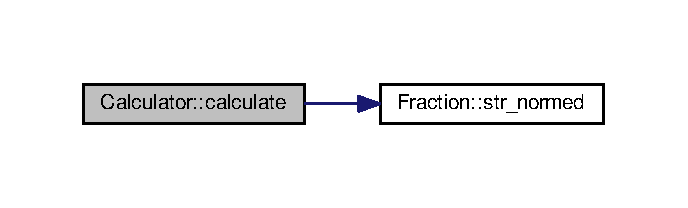
\includegraphics[width=330pt]{classCalculator_ad7c285bf5752406a7cb31e2d215785cc_cgraph}
\end{center}
\end{figure}


\hypertarget{classCalculator_aa1206e4ba90ec9b16996a7719a0b7a6b}{\index{Calculator@{Calculator}!calculate@{calculate}}
\index{calculate@{calculate}!Calculator@{Calculator}}
\subsubsection[{calculate}]{\setlength{\rightskip}{0pt plus 5cm}void Calculator\-::calculate (
\begin{DoxyParamCaption}
\item[{int}]{left, }
\item[{{\bf Fraction}}]{right, }
\item[{std\-::string}]{op}
\end{DoxyParamCaption}
) const  throw (const std\-::invalid\-\_\-argument)}}\label{classCalculator_aa1206e4ba90ec9b16996a7719a0b7a6b}
Calculates a given operation with a integer and a \hyperlink{classFraction}{Fraction}. Prints out the result to the console.


\begin{DoxyParams}{Parameters}
{\em left} & left integer of the operation. \\
\hline
{\em right} & right \hyperlink{classFraction}{Fraction} of the operation. \\
\hline
{\em op} & operator of the operation.\\
\hline
\end{DoxyParams}

\begin{DoxyExceptions}{Exceptions}
{\em std\-::invalid\-\_\-argument} & exception when the operator op doesn't exists. \\
\hline
\end{DoxyExceptions}


Here is the call graph for this function\-:\nopagebreak
\begin{figure}[H]
\begin{center}
\leavevmode
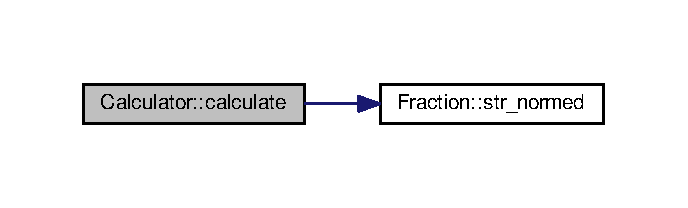
\includegraphics[width=330pt]{classCalculator_aa1206e4ba90ec9b16996a7719a0b7a6b_cgraph}
\end{center}
\end{figure}


\hypertarget{classCalculator_aab2a415730a7a9f0373bf4031fe48acc}{\index{Calculator@{Calculator}!calculate@{calculate}}
\index{calculate@{calculate}!Calculator@{Calculator}}
\subsubsection[{calculate}]{\setlength{\rightskip}{0pt plus 5cm}void Calculator\-::calculate (
\begin{DoxyParamCaption}
\item[{{\bf Fraction}}]{left, }
\item[{int}]{right, }
\item[{std\-::string}]{op}
\end{DoxyParamCaption}
) const  throw (const std\-::invalid\-\_\-argument)}}\label{classCalculator_aab2a415730a7a9f0373bf4031fe48acc}
Calculates a given operation with a \hyperlink{classFraction}{Fraction} and an integer. Prints out the result to the console.


\begin{DoxyParams}{Parameters}
{\em left} & left \hyperlink{classFraction}{Fraction} of the operation. \\
\hline
{\em right} & right integer of the operation. \\
\hline
{\em op} & operator of the operation.\\
\hline
\end{DoxyParams}

\begin{DoxyExceptions}{Exceptions}
{\em invalid\-\_\-argument} & when the operator doesn't exists. \\
\hline
\end{DoxyExceptions}


Here is the call graph for this function\-:\nopagebreak
\begin{figure}[H]
\begin{center}
\leavevmode
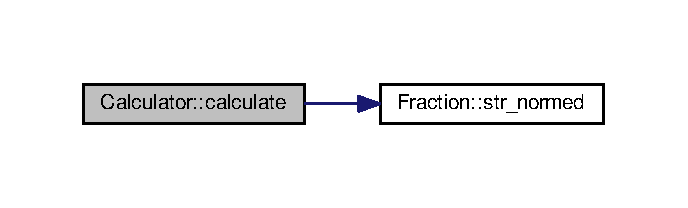
\includegraphics[width=330pt]{classCalculator_aab2a415730a7a9f0373bf4031fe48acc_cgraph}
\end{center}
\end{figure}


\hypertarget{classCalculator_ab63c1adcd80233adf0c75b2fedbc9358}{\index{Calculator@{Calculator}!compare@{compare}}
\index{compare@{compare}!Calculator@{Calculator}}
\subsubsection[{compare}]{\setlength{\rightskip}{0pt plus 5cm}void Calculator\-::compare (
\begin{DoxyParamCaption}
\item[{{\bf Fraction}}]{left, }
\item[{{\bf Fraction}}]{right}
\end{DoxyParamCaption}
) const}}\label{classCalculator_ab63c1adcd80233adf0c75b2fedbc9358}
Compares two Fractions and prints out the result to the console.


\begin{DoxyParams}{Parameters}
{\em left} & First fraction to compare. \\
\hline
{\em right} & Secont \hyperlink{classFraction}{Fraction} to compare. \\
\hline
\end{DoxyParams}


The documentation for this class was generated from the following files\-:\begin{DoxyCompactItemize}
\item 
\hyperlink{calculator_8h}{calculator.\-h}\item 
\hyperlink{calculator_8cpp}{calculator.\-cpp}\end{DoxyCompactItemize}

\hypertarget{classFraction}{\section{Fraction Class Reference}
\label{classFraction}\index{Fraction@{Fraction}}
}


{\ttfamily \#include $<$fraction.\-h$>$}

\subsection*{Public Member Functions}
\begin{DoxyCompactItemize}
\item 
\hyperlink{classFraction_a29efaf0ef03cceab0bfa637e9eea2b7b}{Fraction} ()
\item 
\hyperlink{classFraction_a6e610a7144e0532f65c6ee45ef55727b}{Fraction} (int number)
\item 
\hyperlink{classFraction_a22f64669ffc85d2a58b9d27ae7d6a325}{Fraction} (int a\-\_\-counter, int a\-\_\-denominator)  throw (const std\-::invalid\-\_\-argument)
\item 
\hyperlink{classFraction_ab00b79044cca6774873bdaae713442b9}{Fraction} (int low\-\_\-numerator, int low\-\_\-denominator, int high\-\_\-numerator, int high\-\_\-denominator, long random)  throw (const std\-::invalid\-\_\-argument)
\item 
std\-::string \hyperlink{classFraction_acce62ee78d404b21f2f1d479cd829d3d}{str} () const 
\item 
std\-::string \hyperlink{classFraction_a7381f62ce532529cb447f4edf8f6dbd4}{str\-\_\-normed} () const 
\item 
int \hyperlink{classFraction_a80ad92f94192095396d0722028f050ca}{compare} (const \hyperlink{classFraction}{Fraction} \&other) const 
\item 
\hyperlink{classFraction}{Fraction} \hyperlink{classFraction_ad896accd57d849ed98ee6d72881fcb9d}{operator+} (const \hyperlink{classFraction}{Fraction} \&other) const 
\item 
\hyperlink{classFraction}{Fraction} \hyperlink{classFraction_ad02a7202d1cbc6260a09f9548d061ceb}{operator+} (const int \&number) const 
\item 
\hyperlink{classFraction}{Fraction} \hyperlink{classFraction_a889369a41355240f4f62654d5df52641}{operator-\/} (const \hyperlink{classFraction}{Fraction} \&other) const 
\item 
\hyperlink{classFraction}{Fraction} \hyperlink{classFraction_aac873ae172a2da47085a475322c41905}{operator-\/} (const int \&number) const 
\item 
\hyperlink{classFraction}{Fraction} \hyperlink{classFraction_ab742d856770b1ec746aedf6382ee35df}{operator$\ast$} (const \hyperlink{classFraction}{Fraction} \&other) const 
\item 
\hyperlink{classFraction}{Fraction} \hyperlink{classFraction_adfde5a22f3fe5b0b70c3008162ca014b}{operator$\ast$} (const int \&number) const 
\item 
\hyperlink{classFraction}{Fraction} \hyperlink{classFraction_a572eedd14d4ec9e42a65130029aac360}{operator/} (const \hyperlink{classFraction}{Fraction} \&other) const 
\item 
\hyperlink{classFraction}{Fraction} \hyperlink{classFraction_a81c6eb908f902b21dedcbdf50341d4f4}{operator/} (const int \&number) const   throw (const std\-::invalid\-\_\-argument)
\item 
bool \hyperlink{classFraction_a6c59460c8a1694a99173f1546ee5ffe5}{operator==} (const \hyperlink{classFraction}{Fraction} \&other) const 
\item 
bool \hyperlink{classFraction_ac846064d1566945f66bd7bd0bc6708cf}{operator$<$} (const \hyperlink{classFraction}{Fraction} \&other) const 
\item 
bool \hyperlink{classFraction_a447af586d29a0f0175b608262415698b}{operator$>$} (const \hyperlink{classFraction}{Fraction} \&other) const 
\item 
bool \hyperlink{classFraction_a04fbb8fb0170728e8a0b9c1efe0a9c62}{operator$<$=} (const \hyperlink{classFraction}{Fraction} \&other) const 
\item 
bool \hyperlink{classFraction_a178bbf6662c0ee3bf7e275c65355278a}{operator$>$=} (const \hyperlink{classFraction}{Fraction} \&other) const 
\end{DoxyCompactItemize}


\subsection{Detailed Description}
Implementation of a \hyperlink{classFraction}{Fraction}. Gives the possibility to represent Fractions and calculate with them. As the defaut mathematical operators are overwridden, the class can be used the same way as standard c++ classes.

\begin{DoxyAuthor}{Author}
Lukas Hodel 
\end{DoxyAuthor}
\begin{DoxyVersion}{Version}
1.\-0 
\end{DoxyVersion}


\subsection{Constructor \& Destructor Documentation}
\hypertarget{classFraction_a29efaf0ef03cceab0bfa637e9eea2b7b}{\index{Fraction@{Fraction}!Fraction@{Fraction}}
\index{Fraction@{Fraction}!Fraction@{Fraction}}
\subsubsection[{Fraction}]{\setlength{\rightskip}{0pt plus 5cm}Fraction\-::\-Fraction (
\begin{DoxyParamCaption}
{}
\end{DoxyParamCaption}
)}}\label{classFraction_a29efaf0ef03cceab0bfa637e9eea2b7b}
Initializes a \hyperlink{classFraction}{Fraction} 0/1 which represents 0. \hypertarget{classFraction_a6e610a7144e0532f65c6ee45ef55727b}{\index{Fraction@{Fraction}!Fraction@{Fraction}}
\index{Fraction@{Fraction}!Fraction@{Fraction}}
\subsubsection[{Fraction}]{\setlength{\rightskip}{0pt plus 5cm}Fraction\-::\-Fraction (
\begin{DoxyParamCaption}
\item[{int}]{number}
\end{DoxyParamCaption}
)}}\label{classFraction_a6e610a7144e0532f65c6ee45ef55727b}
Initializes a \hyperlink{classFraction}{Fraction} out of a given integer.


\begin{DoxyParams}{Parameters}
{\em number} & numerator of the \hyperlink{classFraction}{Fraction}. \\
\hline
\end{DoxyParams}
\hypertarget{classFraction_a22f64669ffc85d2a58b9d27ae7d6a325}{\index{Fraction@{Fraction}!Fraction@{Fraction}}
\index{Fraction@{Fraction}!Fraction@{Fraction}}
\subsubsection[{Fraction}]{\setlength{\rightskip}{0pt plus 5cm}Fraction\-::\-Fraction (
\begin{DoxyParamCaption}
\item[{int}]{a\-\_\-numerator, }
\item[{int}]{a\-\_\-denominator}
\end{DoxyParamCaption}
)  throw (const std\-::invalid\-\_\-argument)}}\label{classFraction_a22f64669ffc85d2a58b9d27ae7d6a325}
Initializes a \hyperlink{classFraction}{Fraction} with a given numerator and denominator. numerator / denominator.


\begin{DoxyParams}{Parameters}
{\em a\-\_\-numerator} & numerator of the fraction. \\
\hline
{\em a\-\_\-denominator} & denominator of the \hyperlink{classFraction}{Fraction}.\\
\hline
\end{DoxyParams}

\begin{DoxyExceptions}{Exceptions}
{\em std\-::invalid\-\_\-argument} & when denominator is 0. \\
\hline
\end{DoxyExceptions}
\hypertarget{classFraction_ab00b79044cca6774873bdaae713442b9}{\index{Fraction@{Fraction}!Fraction@{Fraction}}
\index{Fraction@{Fraction}!Fraction@{Fraction}}
\subsubsection[{Fraction}]{\setlength{\rightskip}{0pt plus 5cm}Fraction\-::\-Fraction (
\begin{DoxyParamCaption}
\item[{int}]{low\-\_\-numerator, }
\item[{int}]{low\-\_\-denominator, }
\item[{int}]{high\-\_\-numerator, }
\item[{int}]{high\-\_\-denominator, }
\item[{long}]{random}
\end{DoxyParamCaption}
)  throw (const std\-::invalid\-\_\-argument)}}\label{classFraction_ab00b79044cca6774873bdaae713442b9}
Initializes a random \hyperlink{classFraction}{Fraction} between the Fractions low\-\_\-numerator/low\-\_\-denumerator and high\-\_\-numerator/high\-\_\-denominator.


\begin{DoxyParams}{Parameters}
{\em low\-\_\-numerator} & numerator of the lower bound \hyperlink{classFraction}{Fraction}. \\
\hline
{\em low\-\_\-denominator} & denominator of the lower bound \hyperlink{classFraction}{Fraction}. \\
\hline
{\em high\-\_\-numerator} & numerator of the higher bound \hyperlink{classFraction}{Fraction}. \\
\hline
{\em high\-\_\-denominator} & denominator of the higher boud \hyperlink{classFraction}{Fraction}. \\
\hline
{\em random} & a random number for example the result of rand().\\
\hline
\end{DoxyParams}

\begin{DoxyExceptions}{Exceptions}
{\em std\-::invalid\-\_\-argument} & when low\-\_\-denominator or high\-\_\-denominator is 0. \\
\hline
\end{DoxyExceptions}


\subsection{Member Function Documentation}
\hypertarget{classFraction_a80ad92f94192095396d0722028f050ca}{\index{Fraction@{Fraction}!compare@{compare}}
\index{compare@{compare}!Fraction@{Fraction}}
\subsubsection[{compare}]{\setlength{\rightskip}{0pt plus 5cm}int Fraction\-::compare (
\begin{DoxyParamCaption}
\item[{const {\bf Fraction} \&}]{other}
\end{DoxyParamCaption}
) const}}\label{classFraction_a80ad92f94192095396d0722028f050ca}
Compares the \hyperlink{classFraction}{Fraction} with an other \hyperlink{classFraction}{Fraction}.


\begin{DoxyParams}{Parameters}
{\em other} & Other \hyperlink{classFraction}{Fraction} to compare with the \hyperlink{classFraction}{Fraction}.\\
\hline
\end{DoxyParams}
\begin{DoxyReturn}{Returns}
0 \hyperlink{classFraction}{Fraction} have the same value. 1 \hyperlink{classFraction}{Fraction} is bigger then other \hyperlink{classFraction}{Fraction}. -\/1 \hyperlink{classFraction}{Fraction} is smaller than other facton. 
\end{DoxyReturn}
\hypertarget{classFraction_ab742d856770b1ec746aedf6382ee35df}{\index{Fraction@{Fraction}!operator$\ast$@{operator$\ast$}}
\index{operator$\ast$@{operator$\ast$}!Fraction@{Fraction}}
\subsubsection[{operator$\ast$}]{\setlength{\rightskip}{0pt plus 5cm}{\bf Fraction} Fraction\-::operator$\ast$ (
\begin{DoxyParamCaption}
\item[{const {\bf Fraction} \&}]{other}
\end{DoxyParamCaption}
) const}}\label{classFraction_ab742d856770b1ec746aedf6382ee35df}
Overloading of the operator$\ast$. Defines the multiplication of two Fractions.


\begin{DoxyParams}{Parameters}
{\em other} & Other \hyperlink{classFraction}{Fraction} to multiply to the \hyperlink{classFraction}{Fraction}.\\
\hline
\end{DoxyParams}
\begin{DoxyReturn}{Returns}
a new \hyperlink{classFraction}{Fraction} representing the multiplication of the two \hyperlink{classFraction}{Fraction}. 
\end{DoxyReturn}
\hypertarget{classFraction_adfde5a22f3fe5b0b70c3008162ca014b}{\index{Fraction@{Fraction}!operator$\ast$@{operator$\ast$}}
\index{operator$\ast$@{operator$\ast$}!Fraction@{Fraction}}
\subsubsection[{operator$\ast$}]{\setlength{\rightskip}{0pt plus 5cm}{\bf Fraction} Fraction\-::operator$\ast$ (
\begin{DoxyParamCaption}
\item[{const int \&}]{number}
\end{DoxyParamCaption}
) const}}\label{classFraction_adfde5a22f3fe5b0b70c3008162ca014b}
Overloading of the operator$\ast$. Defines the multiplication of a \hyperlink{classFraction}{Fraction} and a number.


\begin{DoxyParams}{Parameters}
{\em number} & The number to multiply to the \hyperlink{classFraction}{Fraction}.\\
\hline
\end{DoxyParams}
\begin{DoxyReturn}{Returns}
a new \hyperlink{classFraction}{Fraction} with the diffecence of the number and the \hyperlink{classFraction}{Fraction}. 
\end{DoxyReturn}
\hypertarget{classFraction_ad896accd57d849ed98ee6d72881fcb9d}{\index{Fraction@{Fraction}!operator+@{operator+}}
\index{operator+@{operator+}!Fraction@{Fraction}}
\subsubsection[{operator+}]{\setlength{\rightskip}{0pt plus 5cm}{\bf Fraction} Fraction\-::operator+ (
\begin{DoxyParamCaption}
\item[{const {\bf Fraction} \&}]{other}
\end{DoxyParamCaption}
) const}}\label{classFraction_ad896accd57d849ed98ee6d72881fcb9d}
Overloading of the operator+. Defines the addition of two Fractions.


\begin{DoxyParams}{Parameters}
{\em other} & Other \hyperlink{classFraction}{Fraction} to add to the \hyperlink{classFraction}{Fraction}.\\
\hline
\end{DoxyParams}
\begin{DoxyReturn}{Returns}
a new \hyperlink{classFraction}{Fraction} representing the sum of the two \hyperlink{classFraction}{Fraction}. 
\end{DoxyReturn}
\hypertarget{classFraction_ad02a7202d1cbc6260a09f9548d061ceb}{\index{Fraction@{Fraction}!operator+@{operator+}}
\index{operator+@{operator+}!Fraction@{Fraction}}
\subsubsection[{operator+}]{\setlength{\rightskip}{0pt plus 5cm}{\bf Fraction} Fraction\-::operator+ (
\begin{DoxyParamCaption}
\item[{const int \&}]{number}
\end{DoxyParamCaption}
) const}}\label{classFraction_ad02a7202d1cbc6260a09f9548d061ceb}
Overloading of the operator+. Defines the addition of a \hyperlink{classFraction}{Fraction} and a number.


\begin{DoxyParams}{Parameters}
{\em number} & The number to add to the \hyperlink{classFraction}{Fraction}.\\
\hline
\end{DoxyParams}
\begin{DoxyReturn}{Returns}
a new \hyperlink{classFraction}{Fraction} with the sum of the number and the \hyperlink{classFraction}{Fraction}. 
\end{DoxyReturn}
\hypertarget{classFraction_a889369a41355240f4f62654d5df52641}{\index{Fraction@{Fraction}!operator-\/@{operator-\/}}
\index{operator-\/@{operator-\/}!Fraction@{Fraction}}
\subsubsection[{operator-\/}]{\setlength{\rightskip}{0pt plus 5cm}{\bf Fraction} Fraction\-::operator-\/ (
\begin{DoxyParamCaption}
\item[{const {\bf Fraction} \&}]{other}
\end{DoxyParamCaption}
) const}}\label{classFraction_a889369a41355240f4f62654d5df52641}
Overloading of the operator-\/. Defines the subtraction of two Fractions.


\begin{DoxyParams}{Parameters}
{\em other} & Other \hyperlink{classFraction}{Fraction} to subtract to the \hyperlink{classFraction}{Fraction}.\\
\hline
\end{DoxyParams}
\begin{DoxyReturn}{Returns}
a new \hyperlink{classFraction}{Fraction} with the difference of the two \hyperlink{classFraction}{Fraction}. 
\end{DoxyReturn}
\hypertarget{classFraction_aac873ae172a2da47085a475322c41905}{\index{Fraction@{Fraction}!operator-\/@{operator-\/}}
\index{operator-\/@{operator-\/}!Fraction@{Fraction}}
\subsubsection[{operator-\/}]{\setlength{\rightskip}{0pt plus 5cm}{\bf Fraction} Fraction\-::operator-\/ (
\begin{DoxyParamCaption}
\item[{const int \&}]{number}
\end{DoxyParamCaption}
) const}}\label{classFraction_aac873ae172a2da47085a475322c41905}
Overloading of the operator-\/. Defines the subtraction of a \hyperlink{classFraction}{Fraction} and a number.


\begin{DoxyParams}{Parameters}
{\em number} & The number to subtract to the \hyperlink{classFraction}{Fraction}.\\
\hline
\end{DoxyParams}
\begin{DoxyReturn}{Returns}
a new \hyperlink{classFraction}{Fraction} with the diffecence of the number and the \hyperlink{classFraction}{Fraction}. 
\end{DoxyReturn}
\hypertarget{classFraction_a572eedd14d4ec9e42a65130029aac360}{\index{Fraction@{Fraction}!operator/@{operator/}}
\index{operator/@{operator/}!Fraction@{Fraction}}
\subsubsection[{operator/}]{\setlength{\rightskip}{0pt plus 5cm}{\bf Fraction} Fraction\-::operator/ (
\begin{DoxyParamCaption}
\item[{const {\bf Fraction} \&}]{other}
\end{DoxyParamCaption}
) const}}\label{classFraction_a572eedd14d4ec9e42a65130029aac360}
Overloading of the operator/. Defines the division of two Fractions.


\begin{DoxyParams}{Parameters}
{\em other} & Other \hyperlink{classFraction}{Fraction} to divide the \hyperlink{classFraction}{Fraction} with.\\
\hline
\end{DoxyParams}
\begin{DoxyReturn}{Returns}
a new \hyperlink{classFraction}{Fraction} with the quotion form the division of the \hyperlink{classFraction}{Fraction} with the other (right) \hyperlink{classFraction}{Fraction}. 
\end{DoxyReturn}


Here is the call graph for this function\-:\nopagebreak
\begin{figure}[H]
\begin{center}
\leavevmode
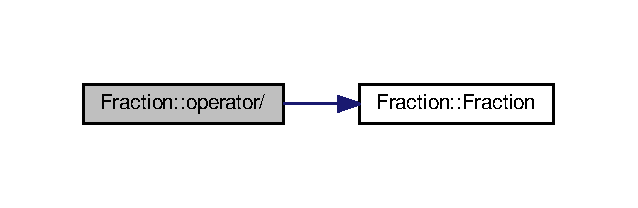
\includegraphics[width=306pt]{classFraction_a572eedd14d4ec9e42a65130029aac360_cgraph}
\end{center}
\end{figure}


\hypertarget{classFraction_a81c6eb908f902b21dedcbdf50341d4f4}{\index{Fraction@{Fraction}!operator/@{operator/}}
\index{operator/@{operator/}!Fraction@{Fraction}}
\subsubsection[{operator/}]{\setlength{\rightskip}{0pt plus 5cm}{\bf Fraction} Fraction\-::operator/ (
\begin{DoxyParamCaption}
\item[{const int \&}]{number}
\end{DoxyParamCaption}
) const  throw (const std\-::invalid\-\_\-argument)}}\label{classFraction_a81c6eb908f902b21dedcbdf50341d4f4}
Overloading of the operator/. Defines the division of a \hyperlink{classFraction}{Fraction} and a number.


\begin{DoxyParams}{Parameters}
{\em number} & The number to devide the \hyperlink{classFraction}{Fraction} with.\\
\hline
\end{DoxyParams}
\begin{DoxyReturn}{Returns}
a new \hyperlink{classFraction}{Fraction} with the quotion from the division of the \hyperlink{classFraction}{Fraction} with the number (right).
\end{DoxyReturn}

\begin{DoxyExceptions}{Exceptions}
{\em std\-::invalid\-\_\-argument} & when divisor number is 0. \\
\hline
\end{DoxyExceptions}
\hypertarget{classFraction_ac846064d1566945f66bd7bd0bc6708cf}{\index{Fraction@{Fraction}!operator$<$@{operator$<$}}
\index{operator$<$@{operator$<$}!Fraction@{Fraction}}
\subsubsection[{operator$<$}]{\setlength{\rightskip}{0pt plus 5cm}bool Fraction\-::operator$<$ (
\begin{DoxyParamCaption}
\item[{const {\bf Fraction} \&}]{other}
\end{DoxyParamCaption}
) const}}\label{classFraction_ac846064d1566945f66bd7bd0bc6708cf}
Defines when a \hyperlink{classFraction}{Fraction} is smaller than an other \hyperlink{classFraction}{Fraction}.


\begin{DoxyParams}{Parameters}
{\em other} & Other \hyperlink{classFraction}{Fraction} to compare \char`\"{}smaller then\char`\"{}\\
\hline
\end{DoxyParams}
\begin{DoxyReturn}{Returns}
true when the \hyperlink{classFraction}{Fraction} is smaller than the other \hyperlink{classFraction}{Fraction}. 
\end{DoxyReturn}


Here is the call graph for this function\-:\nopagebreak
\begin{figure}[H]
\begin{center}
\leavevmode
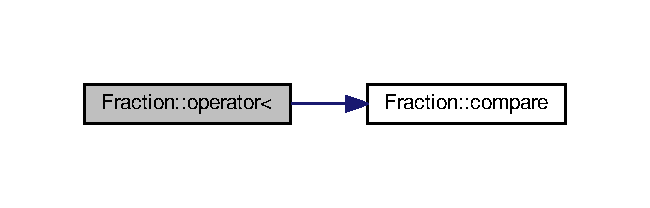
\includegraphics[width=312pt]{classFraction_ac846064d1566945f66bd7bd0bc6708cf_cgraph}
\end{center}
\end{figure}


\hypertarget{classFraction_a04fbb8fb0170728e8a0b9c1efe0a9c62}{\index{Fraction@{Fraction}!operator$<$=@{operator$<$=}}
\index{operator$<$=@{operator$<$=}!Fraction@{Fraction}}
\subsubsection[{operator$<$=}]{\setlength{\rightskip}{0pt plus 5cm}bool Fraction\-::operator$<$= (
\begin{DoxyParamCaption}
\item[{const {\bf Fraction} \&}]{other}
\end{DoxyParamCaption}
) const}}\label{classFraction_a04fbb8fb0170728e8a0b9c1efe0a9c62}
Defines when a \hyperlink{classFraction}{Fraction} is smaller or equal than an other \hyperlink{classFraction}{Fraction}.


\begin{DoxyParams}{Parameters}
{\em other} & Other \hyperlink{classFraction}{Fraction} to compare \char`\"{}smaller or equal than\char`\"{}\\
\hline
\end{DoxyParams}
\begin{DoxyReturn}{Returns}
true when the \hyperlink{classFraction}{Fraction} is smaller or equal than the other \hyperlink{classFraction}{Fraction}. false when the \hyperlink{classFraction}{Fraction} is bigger than the other \hyperlink{classFraction}{Fraction}. 
\end{DoxyReturn}
\hypertarget{classFraction_a6c59460c8a1694a99173f1546ee5ffe5}{\index{Fraction@{Fraction}!operator==@{operator==}}
\index{operator==@{operator==}!Fraction@{Fraction}}
\subsubsection[{operator==}]{\setlength{\rightskip}{0pt plus 5cm}bool Fraction\-::operator== (
\begin{DoxyParamCaption}
\item[{const {\bf Fraction} \&}]{other}
\end{DoxyParamCaption}
) const}}\label{classFraction_a6c59460c8a1694a99173f1546ee5ffe5}
Defines the equalness of two Fractions.


\begin{DoxyParams}{Parameters}
{\em other} & The other \hyperlink{classFraction}{Fraction} to compare equalness.\\
\hline
\end{DoxyParams}
\begin{DoxyReturn}{Returns}
true The fractions are equal, represent the same rational number. false The Fractions are not equal. 
\end{DoxyReturn}


Here is the call graph for this function\-:\nopagebreak
\begin{figure}[H]
\begin{center}
\leavevmode
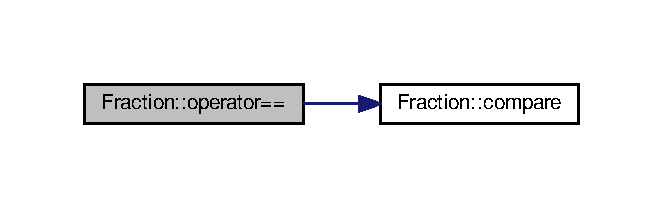
\includegraphics[width=318pt]{classFraction_a6c59460c8a1694a99173f1546ee5ffe5_cgraph}
\end{center}
\end{figure}


\hypertarget{classFraction_a447af586d29a0f0175b608262415698b}{\index{Fraction@{Fraction}!operator$>$@{operator$>$}}
\index{operator$>$@{operator$>$}!Fraction@{Fraction}}
\subsubsection[{operator$>$}]{\setlength{\rightskip}{0pt plus 5cm}bool Fraction\-::operator$>$ (
\begin{DoxyParamCaption}
\item[{const {\bf Fraction} \&}]{other}
\end{DoxyParamCaption}
) const}}\label{classFraction_a447af586d29a0f0175b608262415698b}
Defines when a \hyperlink{classFraction}{Fraction} is bigger than an other \hyperlink{classFraction}{Fraction}.


\begin{DoxyParams}{Parameters}
{\em other} & Other \hyperlink{classFraction}{Fraction} to compare \char`\"{}bigger then\char`\"{}\\
\hline
\end{DoxyParams}
\begin{DoxyReturn}{Returns}
true when the \hyperlink{classFraction}{Fraction} is bigger than the other \hyperlink{classFraction}{Fraction}. false when the \hyperlink{classFraction}{Fraction} is smaller or equal than the other \hyperlink{classFraction}{Fraction}. 
\end{DoxyReturn}
\hypertarget{classFraction_a178bbf6662c0ee3bf7e275c65355278a}{\index{Fraction@{Fraction}!operator$>$=@{operator$>$=}}
\index{operator$>$=@{operator$>$=}!Fraction@{Fraction}}
\subsubsection[{operator$>$=}]{\setlength{\rightskip}{0pt plus 5cm}bool Fraction\-::operator$>$= (
\begin{DoxyParamCaption}
\item[{const {\bf Fraction} \&}]{other}
\end{DoxyParamCaption}
) const}}\label{classFraction_a178bbf6662c0ee3bf7e275c65355278a}
Defines when a \hyperlink{classFraction}{Fraction} is bigger or equal than an other \hyperlink{classFraction}{Fraction}.


\begin{DoxyParams}{Parameters}
{\em other} & Other \hyperlink{classFraction}{Fraction} to compare \char`\"{}bigger or equal than\char`\"{}\\
\hline
\end{DoxyParams}
\begin{DoxyReturn}{Returns}
true when the \hyperlink{classFraction}{Fraction} is bigger or equal than the other \hyperlink{classFraction}{Fraction}. false when the \hyperlink{classFraction}{Fraction} is smaller han the other \hyperlink{classFraction}{Fraction}. 
\end{DoxyReturn}
\hypertarget{classFraction_acce62ee78d404b21f2f1d479cd829d3d}{\index{Fraction@{Fraction}!str@{str}}
\index{str@{str}!Fraction@{Fraction}}
\subsubsection[{str}]{\setlength{\rightskip}{0pt plus 5cm}std\-::string Fraction\-::str (
\begin{DoxyParamCaption}
{}
\end{DoxyParamCaption}
) const}}\label{classFraction_acce62ee78d404b21f2f1d479cd829d3d}
Returns the \hyperlink{classFraction}{Fraction} as a string.

\begin{DoxyReturn}{Returns}
\hyperlink{classFraction}{Fraction} as a string \char`\"{}nominator/denominator\char`\"{} 
\end{DoxyReturn}
\hypertarget{classFraction_a7381f62ce532529cb447f4edf8f6dbd4}{\index{Fraction@{Fraction}!str\-\_\-normed@{str\-\_\-normed}}
\index{str\-\_\-normed@{str\-\_\-normed}!Fraction@{Fraction}}
\subsubsection[{str\-\_\-normed}]{\setlength{\rightskip}{0pt plus 5cm}std\-::string Fraction\-::str\-\_\-normed (
\begin{DoxyParamCaption}
{}
\end{DoxyParamCaption}
) const}}\label{classFraction_a7381f62ce532529cb447f4edf8f6dbd4}
Returns the \hyperlink{classFraction}{Fraction} as a nomed string. 0/1 =$>$ 0 1/1, 3/3, ... =$>$ 1

\begin{DoxyReturn}{Returns}
\hyperlink{classFraction}{Fraction} as a normed string. 
\end{DoxyReturn}


The documentation for this class was generated from the following files\-:\begin{DoxyCompactItemize}
\item 
\hyperlink{fraction_8h}{fraction.\-h}\item 
\hyperlink{fraction_8cpp}{fraction.\-cpp}\end{DoxyCompactItemize}

\chapter{File Documentation}
\hypertarget{calculator_8cpp}{\section{calculator.\-cpp File Reference}
\label{calculator_8cpp}\index{calculator.\-cpp@{calculator.\-cpp}}
}
{\ttfamily \#include $<$iostream$>$}\\*
{\ttfamily \#include $<$string$>$}\\*
{\ttfamily \#include $<$stdexcept$>$}\\*
{\ttfamily \#include \char`\"{}fraction.\-h\char`\"{}}\\*
{\ttfamily \#include \char`\"{}calculator.\-h\char`\"{}}\\*
Include dependency graph for calculator.\-cpp\-:\nopagebreak
\begin{figure}[H]
\begin{center}
\leavevmode
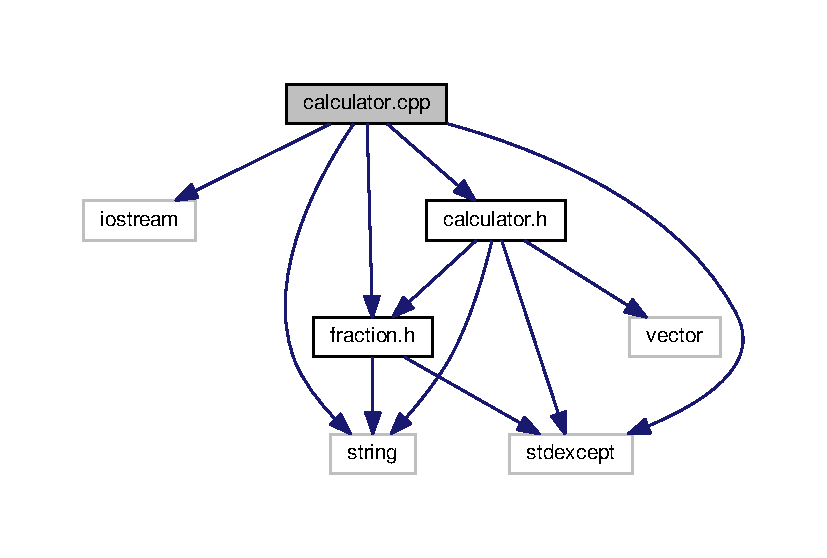
\includegraphics[width=350pt]{calculator_8cpp__incl}
\end{center}
\end{figure}

\hypertarget{calculator_8h}{\section{calculator.\-h File Reference}
\label{calculator_8h}\index{calculator.\-h@{calculator.\-h}}
}
{\ttfamily \#include $<$string$>$}\\*
{\ttfamily \#include $<$vector$>$}\\*
{\ttfamily \#include $<$stdexcept$>$}\\*
{\ttfamily \#include \char`\"{}fraction.\-h\char`\"{}}\\*
Include dependency graph for calculator.\-h\-:\nopagebreak
\begin{figure}[H]
\begin{center}
\leavevmode
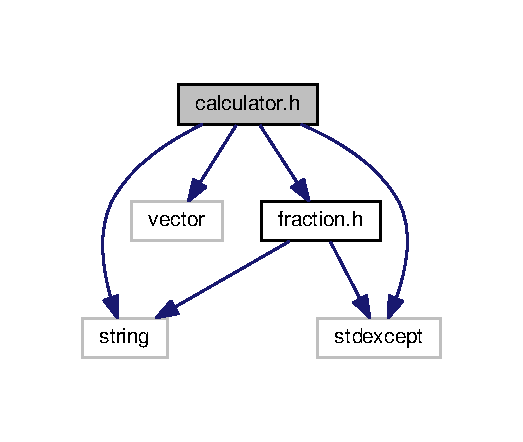
\includegraphics[width=251pt]{calculator_8h__incl}
\end{center}
\end{figure}
This graph shows which files directly or indirectly include this file\-:\nopagebreak
\begin{figure}[H]
\begin{center}
\leavevmode
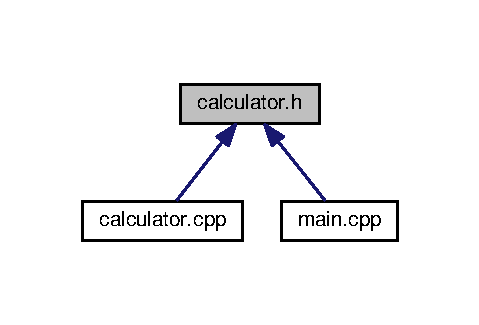
\includegraphics[width=230pt]{calculator_8h__dep__incl}
\end{center}
\end{figure}
\subsection*{Classes}
\begin{DoxyCompactItemize}
\item 
class \hyperlink{classCalculator}{Calculator}
\end{DoxyCompactItemize}
\subsection*{Typedefs}
\begin{DoxyCompactItemize}
\item 
typedef \hyperlink{classFraction}{Fraction}(Fraction\-::$\ast$ \hyperlink{calculator_8h_a9b6408a5e81c4f9a51ed827e8c7ca6b3}{fptr} )(const \hyperlink{classFraction}{Fraction} \&) const 
\item 
typedef \hyperlink{classFraction}{Fraction}(Fraction\-::$\ast$ \hyperlink{calculator_8h_a418b3bd910bac84dd93361a1c0400690}{fptr2} )(const int \&) const 
\item 
typedef \hyperlink{classFraction}{Fraction}($\ast$ \hyperlink{calculator_8h_aa046d174f627935ab5810e02c246e7b3}{fptr3} )(const int \&, const \hyperlink{classFraction}{Fraction} \&)
\end{DoxyCompactItemize}


\subsection{Typedef Documentation}
\hypertarget{calculator_8h_a9b6408a5e81c4f9a51ed827e8c7ca6b3}{\index{calculator.\-h@{calculator.\-h}!fptr@{fptr}}
\index{fptr@{fptr}!calculator.h@{calculator.\-h}}
\subsubsection[{fptr}]{\setlength{\rightskip}{0pt plus 5cm}typedef {\bf Fraction}(Fraction\-::$\ast$ fptr)(const {\bf Fraction} \&) const }}\label{calculator_8h_a9b6408a5e81c4f9a51ed827e8c7ca6b3}
\hypertarget{calculator_8h_a418b3bd910bac84dd93361a1c0400690}{\index{calculator.\-h@{calculator.\-h}!fptr2@{fptr2}}
\index{fptr2@{fptr2}!calculator.h@{calculator.\-h}}
\subsubsection[{fptr2}]{\setlength{\rightskip}{0pt plus 5cm}typedef {\bf Fraction}(Fraction\-::$\ast$ fptr2)(const int \&) const }}\label{calculator_8h_a418b3bd910bac84dd93361a1c0400690}
\hypertarget{calculator_8h_aa046d174f627935ab5810e02c246e7b3}{\index{calculator.\-h@{calculator.\-h}!fptr3@{fptr3}}
\index{fptr3@{fptr3}!calculator.h@{calculator.\-h}}
\subsubsection[{fptr3}]{\setlength{\rightskip}{0pt plus 5cm}typedef {\bf Fraction}($\ast$ fptr3)(const int \&, const {\bf Fraction} \&)}}\label{calculator_8h_aa046d174f627935ab5810e02c246e7b3}

\hypertarget{console__input_8cpp}{\section{console\-\_\-input.\-cpp File Reference}
\label{console__input_8cpp}\index{console\-\_\-input.\-cpp@{console\-\_\-input.\-cpp}}
}
{\ttfamily \#include $<$iostream$>$}\\*
{\ttfamily \#include $<$limits$>$}\\*
{\ttfamily \#include $<$string$>$}\\*
{\ttfamily \#include \char`\"{}console\-\_\-input.\-h\char`\"{}}\\*
Include dependency graph for console\-\_\-input.\-cpp\-:\nopagebreak
\begin{figure}[H]
\begin{center}
\leavevmode
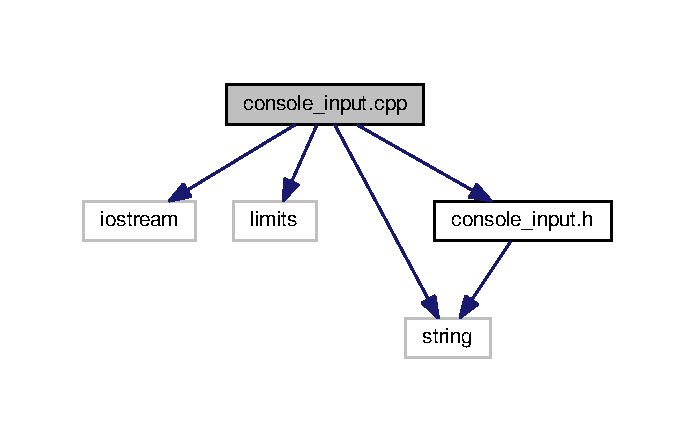
\includegraphics[width=332pt]{console__input_8cpp__incl}
\end{center}
\end{figure}
\subsection*{Functions}
\begin{DoxyCompactItemize}
\item 
double \hyperlink{console__input_8cpp_a8a9df77c5c4adba7ebadb77f3b3dc8ee}{read\-\_\-double} (double min, double max)
\item 
double \hyperlink{console__input_8cpp_a65f2421973540c10e5ae7d10177c566a}{read\-\_\-double} ()
\item 
double \hyperlink{console__input_8cpp_a46878a8594ba71f54911c572031d4614}{read\-\_\-double} (string text)
\item 
double \hyperlink{console__input_8cpp_aca43573be8fe10d4bfede3fc5bd0bd63}{read\-\_\-double} (string text, double min, double max)
\item 
long \hyperlink{console__input_8cpp_a710a686867142de265860584f4147592}{read\-\_\-long} (long min, long max)
\item 
long \hyperlink{console__input_8cpp_a347c616893b725a74f60ea1f7ee325d2}{read\-\_\-long} ()
\item 
long \hyperlink{console__input_8cpp_a9128c63513d87af5259597d8c9930476}{read\-\_\-long} (string text)
\item 
long \hyperlink{console__input_8cpp_a03ebbd2a45117ee03be4e9002210ab36}{read\-\_\-long} (string text, long min, long max)
\item 
int \hyperlink{console__input_8cpp_ad0ccfbb50d0e333ef8acfeab2b7d8071}{read\-\_\-int} (int min, int max)
\item 
int \hyperlink{console__input_8cpp_af310540093ee953c3018bc13bbde3da5}{read\-\_\-int} ()
\item 
int \hyperlink{console__input_8cpp_aaaf3786f6b4803f3120609011de4b0db}{read\-\_\-int} (string text)
\item 
int \hyperlink{console__input_8cpp_a4f8c1bb51d432116d3eda43db3340c8c}{read\-\_\-int} (string text, int min, int max)
\item 
bool \hyperlink{console__input_8cpp_a6bac3909a28fff2736a171022343380b}{read\-\_\-yes\-\_\-no} (string text)
\item 
string \hyperlink{console__input_8cpp_a44ccadd65be527f89bdcf6d27a3b1147}{read\-\_\-text} (string text)
\end{DoxyCompactItemize}


\subsection{Function Documentation}
\hypertarget{console__input_8cpp_a8a9df77c5c4adba7ebadb77f3b3dc8ee}{\index{console\-\_\-input.\-cpp@{console\-\_\-input.\-cpp}!read\-\_\-double@{read\-\_\-double}}
\index{read\-\_\-double@{read\-\_\-double}!console_input.cpp@{console\-\_\-input.\-cpp}}
\subsubsection[{read\-\_\-double}]{\setlength{\rightskip}{0pt plus 5cm}double read\-\_\-double (
\begin{DoxyParamCaption}
\item[{double}]{min, }
\item[{double}]{max}
\end{DoxyParamCaption}
)}}\label{console__input_8cpp_a8a9df77c5c4adba7ebadb77f3b3dc8ee}
Reads a double value in between a given interval from the console. When the entered value is not valid to the interval, the user gets prompted to reenter a valid.


\begin{DoxyParams}{Parameters}
{\em min} & lower bound of the interval. \\
\hline
{\em max} & top bound of the interval\\
\hline
\end{DoxyParams}
\begin{DoxyReturn}{Returns}
a double value in between min and max. 
\end{DoxyReturn}
\hypertarget{console__input_8cpp_a65f2421973540c10e5ae7d10177c566a}{\index{console\-\_\-input.\-cpp@{console\-\_\-input.\-cpp}!read\-\_\-double@{read\-\_\-double}}
\index{read\-\_\-double@{read\-\_\-double}!console_input.cpp@{console\-\_\-input.\-cpp}}
\subsubsection[{read\-\_\-double}]{\setlength{\rightskip}{0pt plus 5cm}double read\-\_\-double (
\begin{DoxyParamCaption}
{}
\end{DoxyParamCaption}
)}}\label{console__input_8cpp_a65f2421973540c10e5ae7d10177c566a}
Reads a double value from the console in between the whole range of double.

\begin{DoxyReturn}{Returns}
a valid double value. 
\end{DoxyReturn}


Here is the call graph for this function\-:\nopagebreak
\begin{figure}[H]
\begin{center}
\leavevmode
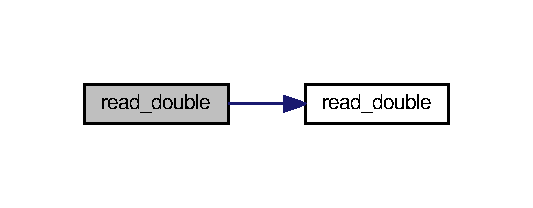
\includegraphics[width=256pt]{console__input_8cpp_a65f2421973540c10e5ae7d10177c566a_cgraph}
\end{center}
\end{figure}


\hypertarget{console__input_8cpp_a46878a8594ba71f54911c572031d4614}{\index{console\-\_\-input.\-cpp@{console\-\_\-input.\-cpp}!read\-\_\-double@{read\-\_\-double}}
\index{read\-\_\-double@{read\-\_\-double}!console_input.cpp@{console\-\_\-input.\-cpp}}
\subsubsection[{read\-\_\-double}]{\setlength{\rightskip}{0pt plus 5cm}double read\-\_\-double (
\begin{DoxyParamCaption}
\item[{string}]{text}
\end{DoxyParamCaption}
)}}\label{console__input_8cpp_a46878a8594ba71f54911c572031d4614}
Prints a text to the console and reads a double value from the console in between the whole range of double.


\begin{DoxyParams}{Parameters}
{\em text} & text to print to the console.\\
\hline
\end{DoxyParams}
\begin{DoxyReturn}{Returns}
a valid double value. 
\end{DoxyReturn}


Here is the call graph for this function\-:\nopagebreak
\begin{figure}[H]
\begin{center}
\leavevmode
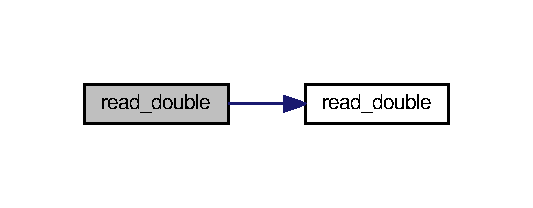
\includegraphics[width=256pt]{console__input_8cpp_a46878a8594ba71f54911c572031d4614_cgraph}
\end{center}
\end{figure}


\hypertarget{console__input_8cpp_aca43573be8fe10d4bfede3fc5bd0bd63}{\index{console\-\_\-input.\-cpp@{console\-\_\-input.\-cpp}!read\-\_\-double@{read\-\_\-double}}
\index{read\-\_\-double@{read\-\_\-double}!console_input.cpp@{console\-\_\-input.\-cpp}}
\subsubsection[{read\-\_\-double}]{\setlength{\rightskip}{0pt plus 5cm}double read\-\_\-double (
\begin{DoxyParamCaption}
\item[{string}]{text, }
\item[{double}]{min, }
\item[{double}]{max}
\end{DoxyParamCaption}
)}}\label{console__input_8cpp_aca43573be8fe10d4bfede3fc5bd0bd63}


Here is the call graph for this function\-:\nopagebreak
\begin{figure}[H]
\begin{center}
\leavevmode
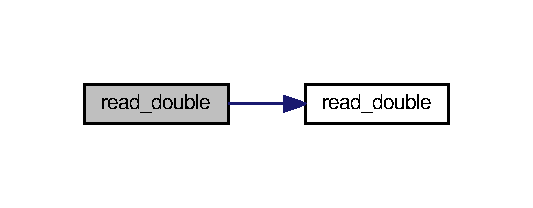
\includegraphics[width=256pt]{console__input_8cpp_aca43573be8fe10d4bfede3fc5bd0bd63_cgraph}
\end{center}
\end{figure}


\hypertarget{console__input_8cpp_ad0ccfbb50d0e333ef8acfeab2b7d8071}{\index{console\-\_\-input.\-cpp@{console\-\_\-input.\-cpp}!read\-\_\-int@{read\-\_\-int}}
\index{read\-\_\-int@{read\-\_\-int}!console_input.cpp@{console\-\_\-input.\-cpp}}
\subsubsection[{read\-\_\-int}]{\setlength{\rightskip}{0pt plus 5cm}int read\-\_\-int (
\begin{DoxyParamCaption}
\item[{int}]{min, }
\item[{int}]{max}
\end{DoxyParamCaption}
)}}\label{console__input_8cpp_ad0ccfbb50d0e333ef8acfeab2b7d8071}
Reads a integer value in between a given interval from the console. When the entered value is not valid to the interval, the user gets prompted to reenter a valid.


\begin{DoxyParams}{Parameters}
{\em min} & lower bound of the interval. \\
\hline
{\em max} & top bound of the interval\\
\hline
\end{DoxyParams}
\begin{DoxyReturn}{Returns}
a int value in between min and max. 
\end{DoxyReturn}


Here is the call graph for this function\-:\nopagebreak
\begin{figure}[H]
\begin{center}
\leavevmode
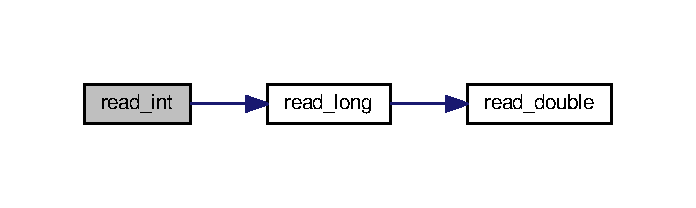
\includegraphics[width=334pt]{console__input_8cpp_ad0ccfbb50d0e333ef8acfeab2b7d8071_cgraph}
\end{center}
\end{figure}


\hypertarget{console__input_8cpp_af310540093ee953c3018bc13bbde3da5}{\index{console\-\_\-input.\-cpp@{console\-\_\-input.\-cpp}!read\-\_\-int@{read\-\_\-int}}
\index{read\-\_\-int@{read\-\_\-int}!console_input.cpp@{console\-\_\-input.\-cpp}}
\subsubsection[{read\-\_\-int}]{\setlength{\rightskip}{0pt plus 5cm}int read\-\_\-int (
\begin{DoxyParamCaption}
{}
\end{DoxyParamCaption}
)}}\label{console__input_8cpp_af310540093ee953c3018bc13bbde3da5}
Reads an integer value from the terminal in between the whole range of long.

\begin{DoxyReturn}{Returns}
a valid integer value. 
\end{DoxyReturn}


Here is the call graph for this function\-:\nopagebreak
\begin{figure}[H]
\begin{center}
\leavevmode
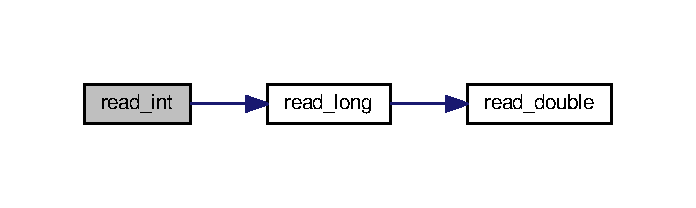
\includegraphics[width=334pt]{console__input_8cpp_af310540093ee953c3018bc13bbde3da5_cgraph}
\end{center}
\end{figure}


\hypertarget{console__input_8cpp_aaaf3786f6b4803f3120609011de4b0db}{\index{console\-\_\-input.\-cpp@{console\-\_\-input.\-cpp}!read\-\_\-int@{read\-\_\-int}}
\index{read\-\_\-int@{read\-\_\-int}!console_input.cpp@{console\-\_\-input.\-cpp}}
\subsubsection[{read\-\_\-int}]{\setlength{\rightskip}{0pt plus 5cm}int read\-\_\-int (
\begin{DoxyParamCaption}
\item[{string}]{text}
\end{DoxyParamCaption}
)}}\label{console__input_8cpp_aaaf3786f6b4803f3120609011de4b0db}
Prints a text to the console and reads a integer value from the console in between the whole range of integer.


\begin{DoxyParams}{Parameters}
{\em text} & text to print to the console.\\
\hline
\end{DoxyParams}
\begin{DoxyReturn}{Returns}
a valid integer value. 
\end{DoxyReturn}


Here is the call graph for this function\-:\nopagebreak
\begin{figure}[H]
\begin{center}
\leavevmode
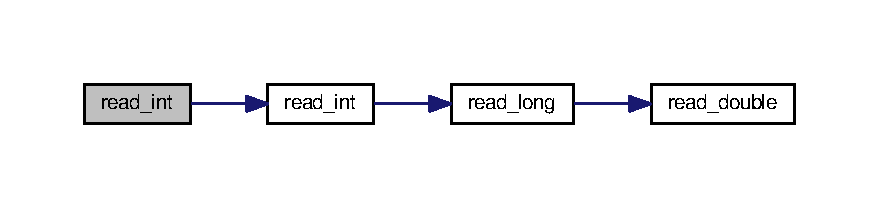
\includegraphics[width=350pt]{console__input_8cpp_aaaf3786f6b4803f3120609011de4b0db_cgraph}
\end{center}
\end{figure}


\hypertarget{console__input_8cpp_a4f8c1bb51d432116d3eda43db3340c8c}{\index{console\-\_\-input.\-cpp@{console\-\_\-input.\-cpp}!read\-\_\-int@{read\-\_\-int}}
\index{read\-\_\-int@{read\-\_\-int}!console_input.cpp@{console\-\_\-input.\-cpp}}
\subsubsection[{read\-\_\-int}]{\setlength{\rightskip}{0pt plus 5cm}int read\-\_\-int (
\begin{DoxyParamCaption}
\item[{string}]{text, }
\item[{int}]{min, }
\item[{int}]{max}
\end{DoxyParamCaption}
)}}\label{console__input_8cpp_a4f8c1bb51d432116d3eda43db3340c8c}
Prints a text to the console and reads a integer value in between a given interval from the console. When the value is not in between the interval, the user gets prompted to reeinter a valid value.


\begin{DoxyParams}{Parameters}
{\em text} & text to print to the console. \\
\hline
{\em min} & lower bound of the interval. \\
\hline
{\em max} & top bound of the interval.\\
\hline
\end{DoxyParams}
\begin{DoxyReturn}{Returns}
a integer value in between min and max. 
\end{DoxyReturn}


Here is the call graph for this function\-:\nopagebreak
\begin{figure}[H]
\begin{center}
\leavevmode
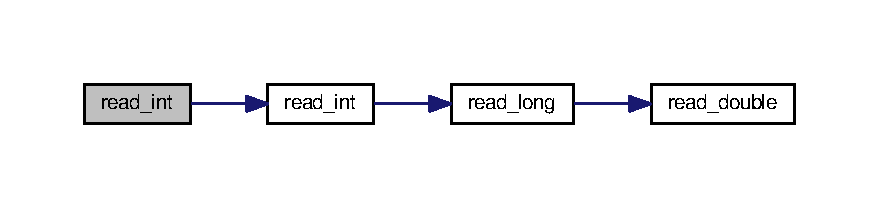
\includegraphics[width=350pt]{console__input_8cpp_a4f8c1bb51d432116d3eda43db3340c8c_cgraph}
\end{center}
\end{figure}


\hypertarget{console__input_8cpp_a710a686867142de265860584f4147592}{\index{console\-\_\-input.\-cpp@{console\-\_\-input.\-cpp}!read\-\_\-long@{read\-\_\-long}}
\index{read\-\_\-long@{read\-\_\-long}!console_input.cpp@{console\-\_\-input.\-cpp}}
\subsubsection[{read\-\_\-long}]{\setlength{\rightskip}{0pt plus 5cm}long read\-\_\-long (
\begin{DoxyParamCaption}
\item[{long}]{min, }
\item[{long}]{max}
\end{DoxyParamCaption}
)}}\label{console__input_8cpp_a710a686867142de265860584f4147592}
Reads a long value in between a given interval from the console. When the entered value is not valid to the interval, the user gets prompted to reenter a valid.


\begin{DoxyParams}{Parameters}
{\em min} & lower bound of the interval. \\
\hline
{\em max} & top bound of the interval\\
\hline
\end{DoxyParams}
\begin{DoxyReturn}{Returns}
a long value in between min and max. 
\end{DoxyReturn}


Here is the call graph for this function\-:\nopagebreak
\begin{figure}[H]
\begin{center}
\leavevmode
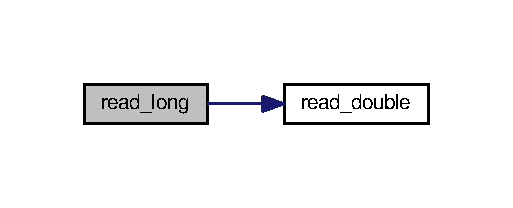
\includegraphics[width=246pt]{console__input_8cpp_a710a686867142de265860584f4147592_cgraph}
\end{center}
\end{figure}


\hypertarget{console__input_8cpp_a347c616893b725a74f60ea1f7ee325d2}{\index{console\-\_\-input.\-cpp@{console\-\_\-input.\-cpp}!read\-\_\-long@{read\-\_\-long}}
\index{read\-\_\-long@{read\-\_\-long}!console_input.cpp@{console\-\_\-input.\-cpp}}
\subsubsection[{read\-\_\-long}]{\setlength{\rightskip}{0pt plus 5cm}long read\-\_\-long (
\begin{DoxyParamCaption}
{}
\end{DoxyParamCaption}
)}}\label{console__input_8cpp_a347c616893b725a74f60ea1f7ee325d2}
Reads a long value from the terminal in between the whole range of long.

\begin{DoxyReturn}{Returns}
a valid long value. 
\end{DoxyReturn}


Here is the call graph for this function\-:\nopagebreak
\begin{figure}[H]
\begin{center}
\leavevmode
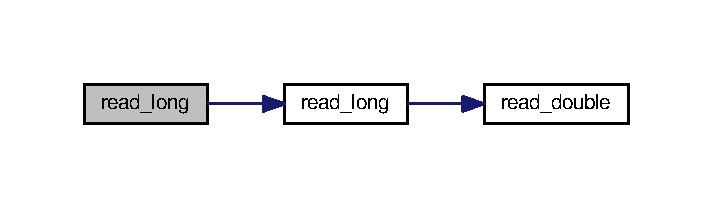
\includegraphics[width=342pt]{console__input_8cpp_a347c616893b725a74f60ea1f7ee325d2_cgraph}
\end{center}
\end{figure}


\hypertarget{console__input_8cpp_a9128c63513d87af5259597d8c9930476}{\index{console\-\_\-input.\-cpp@{console\-\_\-input.\-cpp}!read\-\_\-long@{read\-\_\-long}}
\index{read\-\_\-long@{read\-\_\-long}!console_input.cpp@{console\-\_\-input.\-cpp}}
\subsubsection[{read\-\_\-long}]{\setlength{\rightskip}{0pt plus 5cm}long read\-\_\-long (
\begin{DoxyParamCaption}
\item[{string}]{text}
\end{DoxyParamCaption}
)}}\label{console__input_8cpp_a9128c63513d87af5259597d8c9930476}
Prints a text to the console and reads a long value from the console in between the whole range of long.


\begin{DoxyParams}{Parameters}
{\em text} & text to print to the console.\\
\hline
\end{DoxyParams}
\begin{DoxyReturn}{Returns}
a valid long value. 
\end{DoxyReturn}


Here is the call graph for this function\-:\nopagebreak
\begin{figure}[H]
\begin{center}
\leavevmode
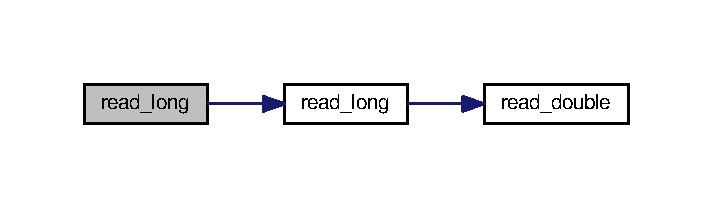
\includegraphics[width=342pt]{console__input_8cpp_a9128c63513d87af5259597d8c9930476_cgraph}
\end{center}
\end{figure}


\hypertarget{console__input_8cpp_a03ebbd2a45117ee03be4e9002210ab36}{\index{console\-\_\-input.\-cpp@{console\-\_\-input.\-cpp}!read\-\_\-long@{read\-\_\-long}}
\index{read\-\_\-long@{read\-\_\-long}!console_input.cpp@{console\-\_\-input.\-cpp}}
\subsubsection[{read\-\_\-long}]{\setlength{\rightskip}{0pt plus 5cm}long read\-\_\-long (
\begin{DoxyParamCaption}
\item[{string}]{text, }
\item[{long}]{min, }
\item[{long}]{max}
\end{DoxyParamCaption}
)}}\label{console__input_8cpp_a03ebbd2a45117ee03be4e9002210ab36}
Prints a text to the console and reads a long value in between a given interval from the console. When the value is not in between the interval, the user gets prompted to reeinter a valid value.


\begin{DoxyParams}{Parameters}
{\em text} & text to print to the console. \\
\hline
{\em min} & lower bound of the interval. \\
\hline
{\em max} & top bound of the interval.\\
\hline
\end{DoxyParams}
\begin{DoxyReturn}{Returns}
a long value in between min and max. 
\end{DoxyReturn}


Here is the call graph for this function\-:\nopagebreak
\begin{figure}[H]
\begin{center}
\leavevmode
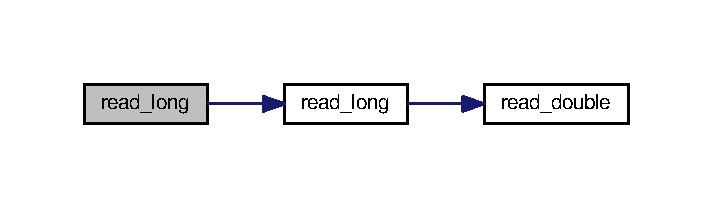
\includegraphics[width=342pt]{console__input_8cpp_a03ebbd2a45117ee03be4e9002210ab36_cgraph}
\end{center}
\end{figure}


\hypertarget{console__input_8cpp_a44ccadd65be527f89bdcf6d27a3b1147}{\index{console\-\_\-input.\-cpp@{console\-\_\-input.\-cpp}!read\-\_\-text@{read\-\_\-text}}
\index{read\-\_\-text@{read\-\_\-text}!console_input.cpp@{console\-\_\-input.\-cpp}}
\subsubsection[{read\-\_\-text}]{\setlength{\rightskip}{0pt plus 5cm}string read\-\_\-text (
\begin{DoxyParamCaption}
\item[{string}]{text}
\end{DoxyParamCaption}
)}}\label{console__input_8cpp_a44ccadd65be527f89bdcf6d27a3b1147}
\hypertarget{console__input_8cpp_a6bac3909a28fff2736a171022343380b}{\index{console\-\_\-input.\-cpp@{console\-\_\-input.\-cpp}!read\-\_\-yes\-\_\-no@{read\-\_\-yes\-\_\-no}}
\index{read\-\_\-yes\-\_\-no@{read\-\_\-yes\-\_\-no}!console_input.cpp@{console\-\_\-input.\-cpp}}
\subsubsection[{read\-\_\-yes\-\_\-no}]{\setlength{\rightskip}{0pt plus 5cm}bool read\-\_\-yes\-\_\-no (
\begin{DoxyParamCaption}
\item[{string}]{text}
\end{DoxyParamCaption}
)}}\label{console__input_8cpp_a6bac3909a28fff2736a171022343380b}

\hypertarget{console__input_8h}{\section{console\-\_\-input.\-h File Reference}
\label{console__input_8h}\index{console\-\_\-input.\-h@{console\-\_\-input.\-h}}
}
{\ttfamily \#include $<$string$>$}\\*
Include dependency graph for console\-\_\-input.\-h\-:\nopagebreak
\begin{figure}[H]
\begin{center}
\leavevmode
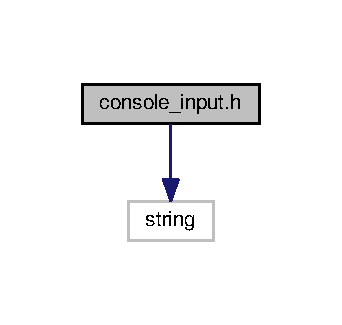
\includegraphics[width=164pt]{console__input_8h__incl}
\end{center}
\end{figure}
This graph shows which files directly or indirectly include this file\-:\nopagebreak
\begin{figure}[H]
\begin{center}
\leavevmode
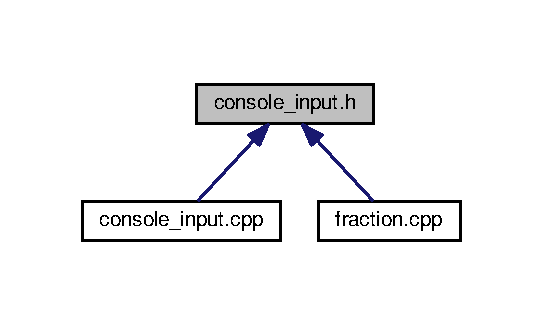
\includegraphics[width=264pt]{console__input_8h__dep__incl}
\end{center}
\end{figure}
\subsection*{Functions}
\begin{DoxyCompactItemize}
\item 
double \hyperlink{console__input_8h_a8a9df77c5c4adba7ebadb77f3b3dc8ee}{read\-\_\-double} (double min, double max)
\item 
double \hyperlink{console__input_8h_a46878a8594ba71f54911c572031d4614}{read\-\_\-double} (string text)
\item 
double \hyperlink{console__input_8h_aca43573be8fe10d4bfede3fc5bd0bd63}{read\-\_\-double} (string text, double min, double max)
\item 
double \hyperlink{console__input_8h_a65f2421973540c10e5ae7d10177c566a}{read\-\_\-double} ()
\item 
void \hyperlink{console__input_8h_afc6e4adf69aec96a5eae4249fbbc7201}{read\-\_\-enter} ()
\item 
long \hyperlink{console__input_8h_a03ebbd2a45117ee03be4e9002210ab36}{read\-\_\-long} (string text, long min, long max)
\item 
long \hyperlink{console__input_8h_a710a686867142de265860584f4147592}{read\-\_\-long} (long min, long max)
\item 
long \hyperlink{console__input_8h_a9128c63513d87af5259597d8c9930476}{read\-\_\-long} (string text)
\item 
long \hyperlink{console__input_8h_a347c616893b725a74f60ea1f7ee325d2}{read\-\_\-long} ()
\item 
int \hyperlink{console__input_8h_a4f8c1bb51d432116d3eda43db3340c8c}{read\-\_\-int} (string text, int min, int max)
\item 
int \hyperlink{console__input_8h_ad0ccfbb50d0e333ef8acfeab2b7d8071}{read\-\_\-int} (int min, int max)
\item 
int \hyperlink{console__input_8h_aaaf3786f6b4803f3120609011de4b0db}{read\-\_\-int} (string text)
\item 
int \hyperlink{console__input_8h_af310540093ee953c3018bc13bbde3da5}{read\-\_\-int} ()
\item 
bool \hyperlink{console__input_8h_a6bac3909a28fff2736a171022343380b}{read\-\_\-yes\-\_\-no} (string text)
\item 
string \hyperlink{console__input_8h_a44ccadd65be527f89bdcf6d27a3b1147}{read\-\_\-text} (string text)
\end{DoxyCompactItemize}


\subsection{Function Documentation}
\hypertarget{console__input_8h_a8a9df77c5c4adba7ebadb77f3b3dc8ee}{\index{console\-\_\-input.\-h@{console\-\_\-input.\-h}!read\-\_\-double@{read\-\_\-double}}
\index{read\-\_\-double@{read\-\_\-double}!console_input.h@{console\-\_\-input.\-h}}
\subsubsection[{read\-\_\-double}]{\setlength{\rightskip}{0pt plus 5cm}double read\-\_\-double (
\begin{DoxyParamCaption}
\item[{double}]{min, }
\item[{double}]{max}
\end{DoxyParamCaption}
)}}\label{console__input_8h_a8a9df77c5c4adba7ebadb77f3b3dc8ee}
Reads a double value in between a given interval from the console. When the entered value is not valid to the interval, the user gets prompted to reenter a valid.


\begin{DoxyParams}{Parameters}
{\em min} & lower bound of the interval. \\
\hline
{\em max} & top bound of the interval\\
\hline
\end{DoxyParams}
\begin{DoxyReturn}{Returns}
a double value in between min and max. 
\end{DoxyReturn}
\hypertarget{console__input_8h_a46878a8594ba71f54911c572031d4614}{\index{console\-\_\-input.\-h@{console\-\_\-input.\-h}!read\-\_\-double@{read\-\_\-double}}
\index{read\-\_\-double@{read\-\_\-double}!console_input.h@{console\-\_\-input.\-h}}
\subsubsection[{read\-\_\-double}]{\setlength{\rightskip}{0pt plus 5cm}double read\-\_\-double (
\begin{DoxyParamCaption}
\item[{string}]{text}
\end{DoxyParamCaption}
)}}\label{console__input_8h_a46878a8594ba71f54911c572031d4614}
Prints a text to the console and reads a double value from the console in between the whole range of double.


\begin{DoxyParams}{Parameters}
{\em text} & text to print to the console.\\
\hline
\end{DoxyParams}
\begin{DoxyReturn}{Returns}
a valid double value. 
\end{DoxyReturn}


Here is the call graph for this function\-:\nopagebreak
\begin{figure}[H]
\begin{center}
\leavevmode
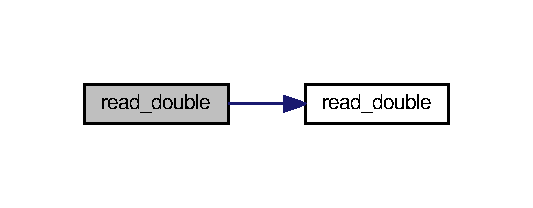
\includegraphics[width=256pt]{console__input_8h_a46878a8594ba71f54911c572031d4614_cgraph}
\end{center}
\end{figure}


\hypertarget{console__input_8h_aca43573be8fe10d4bfede3fc5bd0bd63}{\index{console\-\_\-input.\-h@{console\-\_\-input.\-h}!read\-\_\-double@{read\-\_\-double}}
\index{read\-\_\-double@{read\-\_\-double}!console_input.h@{console\-\_\-input.\-h}}
\subsubsection[{read\-\_\-double}]{\setlength{\rightskip}{0pt plus 5cm}double read\-\_\-double (
\begin{DoxyParamCaption}
\item[{string}]{text, }
\item[{double}]{min, }
\item[{double}]{max}
\end{DoxyParamCaption}
)}}\label{console__input_8h_aca43573be8fe10d4bfede3fc5bd0bd63}


Here is the call graph for this function\-:\nopagebreak
\begin{figure}[H]
\begin{center}
\leavevmode
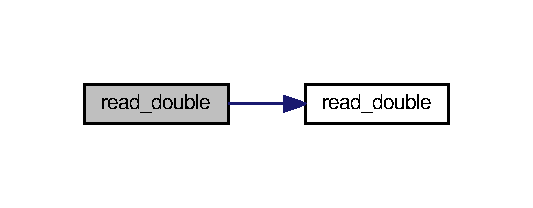
\includegraphics[width=256pt]{console__input_8h_aca43573be8fe10d4bfede3fc5bd0bd63_cgraph}
\end{center}
\end{figure}


\hypertarget{console__input_8h_a65f2421973540c10e5ae7d10177c566a}{\index{console\-\_\-input.\-h@{console\-\_\-input.\-h}!read\-\_\-double@{read\-\_\-double}}
\index{read\-\_\-double@{read\-\_\-double}!console_input.h@{console\-\_\-input.\-h}}
\subsubsection[{read\-\_\-double}]{\setlength{\rightskip}{0pt plus 5cm}double read\-\_\-double (
\begin{DoxyParamCaption}
{}
\end{DoxyParamCaption}
)}}\label{console__input_8h_a65f2421973540c10e5ae7d10177c566a}
Reads a double value from the console in between the whole range of double.

\begin{DoxyReturn}{Returns}
a valid double value. 
\end{DoxyReturn}


Here is the call graph for this function\-:\nopagebreak
\begin{figure}[H]
\begin{center}
\leavevmode
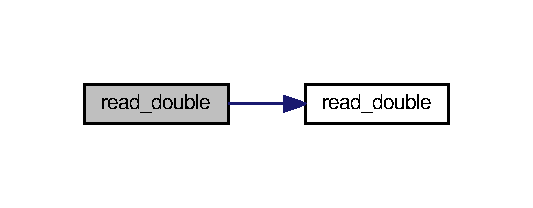
\includegraphics[width=256pt]{console__input_8h_a65f2421973540c10e5ae7d10177c566a_cgraph}
\end{center}
\end{figure}


\hypertarget{console__input_8h_afc6e4adf69aec96a5eae4249fbbc7201}{\index{console\-\_\-input.\-h@{console\-\_\-input.\-h}!read\-\_\-enter@{read\-\_\-enter}}
\index{read\-\_\-enter@{read\-\_\-enter}!console_input.h@{console\-\_\-input.\-h}}
\subsubsection[{read\-\_\-enter}]{\setlength{\rightskip}{0pt plus 5cm}void read\-\_\-enter (
\begin{DoxyParamCaption}
{}
\end{DoxyParamCaption}
)}}\label{console__input_8h_afc6e4adf69aec96a5eae4249fbbc7201}
\hypertarget{console__input_8h_a4f8c1bb51d432116d3eda43db3340c8c}{\index{console\-\_\-input.\-h@{console\-\_\-input.\-h}!read\-\_\-int@{read\-\_\-int}}
\index{read\-\_\-int@{read\-\_\-int}!console_input.h@{console\-\_\-input.\-h}}
\subsubsection[{read\-\_\-int}]{\setlength{\rightskip}{0pt plus 5cm}int read\-\_\-int (
\begin{DoxyParamCaption}
\item[{string}]{text, }
\item[{int}]{min, }
\item[{int}]{max}
\end{DoxyParamCaption}
)}}\label{console__input_8h_a4f8c1bb51d432116d3eda43db3340c8c}
Prints a text to the console and reads a integer value in between a given interval from the console. When the value is not in between the interval, the user gets prompted to reeinter a valid value.


\begin{DoxyParams}{Parameters}
{\em text} & text to print to the console. \\
\hline
{\em min} & lower bound of the interval. \\
\hline
{\em max} & top bound of the interval.\\
\hline
\end{DoxyParams}
\begin{DoxyReturn}{Returns}
a integer value in between min and max. 
\end{DoxyReturn}


Here is the call graph for this function\-:\nopagebreak
\begin{figure}[H]
\begin{center}
\leavevmode
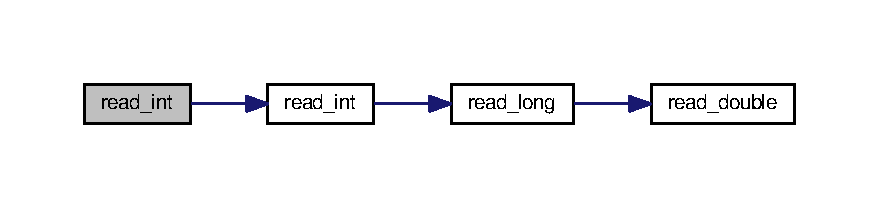
\includegraphics[width=350pt]{console__input_8h_a4f8c1bb51d432116d3eda43db3340c8c_cgraph}
\end{center}
\end{figure}


\hypertarget{console__input_8h_ad0ccfbb50d0e333ef8acfeab2b7d8071}{\index{console\-\_\-input.\-h@{console\-\_\-input.\-h}!read\-\_\-int@{read\-\_\-int}}
\index{read\-\_\-int@{read\-\_\-int}!console_input.h@{console\-\_\-input.\-h}}
\subsubsection[{read\-\_\-int}]{\setlength{\rightskip}{0pt plus 5cm}int read\-\_\-int (
\begin{DoxyParamCaption}
\item[{int}]{min, }
\item[{int}]{max}
\end{DoxyParamCaption}
)}}\label{console__input_8h_ad0ccfbb50d0e333ef8acfeab2b7d8071}
Reads a integer value in between a given interval from the console. When the entered value is not valid to the interval, the user gets prompted to reenter a valid.


\begin{DoxyParams}{Parameters}
{\em min} & lower bound of the interval. \\
\hline
{\em max} & top bound of the interval\\
\hline
\end{DoxyParams}
\begin{DoxyReturn}{Returns}
a int value in between min and max. 
\end{DoxyReturn}


Here is the call graph for this function\-:\nopagebreak
\begin{figure}[H]
\begin{center}
\leavevmode
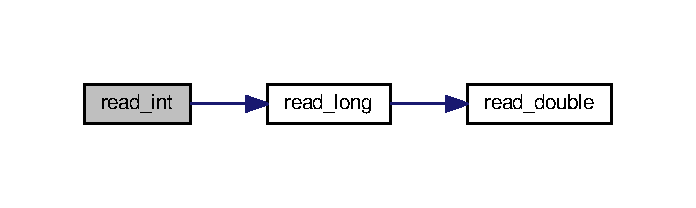
\includegraphics[width=334pt]{console__input_8h_ad0ccfbb50d0e333ef8acfeab2b7d8071_cgraph}
\end{center}
\end{figure}


\hypertarget{console__input_8h_aaaf3786f6b4803f3120609011de4b0db}{\index{console\-\_\-input.\-h@{console\-\_\-input.\-h}!read\-\_\-int@{read\-\_\-int}}
\index{read\-\_\-int@{read\-\_\-int}!console_input.h@{console\-\_\-input.\-h}}
\subsubsection[{read\-\_\-int}]{\setlength{\rightskip}{0pt plus 5cm}int read\-\_\-int (
\begin{DoxyParamCaption}
\item[{string}]{text}
\end{DoxyParamCaption}
)}}\label{console__input_8h_aaaf3786f6b4803f3120609011de4b0db}
Prints a text to the console and reads a integer value from the console in between the whole range of integer.


\begin{DoxyParams}{Parameters}
{\em text} & text to print to the console.\\
\hline
\end{DoxyParams}
\begin{DoxyReturn}{Returns}
a valid integer value. 
\end{DoxyReturn}


Here is the call graph for this function\-:\nopagebreak
\begin{figure}[H]
\begin{center}
\leavevmode
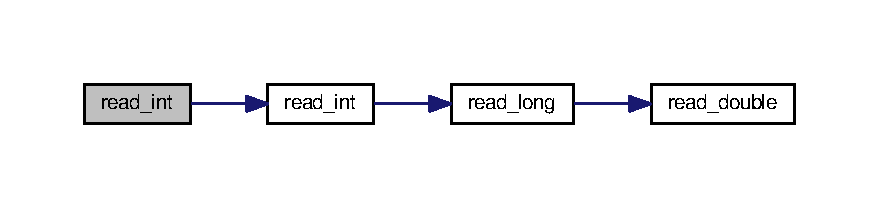
\includegraphics[width=350pt]{console__input_8h_aaaf3786f6b4803f3120609011de4b0db_cgraph}
\end{center}
\end{figure}


\hypertarget{console__input_8h_af310540093ee953c3018bc13bbde3da5}{\index{console\-\_\-input.\-h@{console\-\_\-input.\-h}!read\-\_\-int@{read\-\_\-int}}
\index{read\-\_\-int@{read\-\_\-int}!console_input.h@{console\-\_\-input.\-h}}
\subsubsection[{read\-\_\-int}]{\setlength{\rightskip}{0pt plus 5cm}int read\-\_\-int (
\begin{DoxyParamCaption}
{}
\end{DoxyParamCaption}
)}}\label{console__input_8h_af310540093ee953c3018bc13bbde3da5}
Reads an integer value from the terminal in between the whole range of long.

\begin{DoxyReturn}{Returns}
a valid integer value. 
\end{DoxyReturn}


Here is the call graph for this function\-:\nopagebreak
\begin{figure}[H]
\begin{center}
\leavevmode
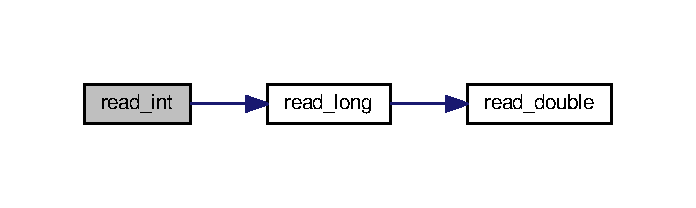
\includegraphics[width=334pt]{console__input_8h_af310540093ee953c3018bc13bbde3da5_cgraph}
\end{center}
\end{figure}


\hypertarget{console__input_8h_a03ebbd2a45117ee03be4e9002210ab36}{\index{console\-\_\-input.\-h@{console\-\_\-input.\-h}!read\-\_\-long@{read\-\_\-long}}
\index{read\-\_\-long@{read\-\_\-long}!console_input.h@{console\-\_\-input.\-h}}
\subsubsection[{read\-\_\-long}]{\setlength{\rightskip}{0pt plus 5cm}long read\-\_\-long (
\begin{DoxyParamCaption}
\item[{string}]{text, }
\item[{long}]{min, }
\item[{long}]{max}
\end{DoxyParamCaption}
)}}\label{console__input_8h_a03ebbd2a45117ee03be4e9002210ab36}
Prints a text to the console and reads a long value in between a given interval from the console. When the value is not in between the interval, the user gets prompted to reeinter a valid value.


\begin{DoxyParams}{Parameters}
{\em text} & text to print to the console. \\
\hline
{\em min} & lower bound of the interval. \\
\hline
{\em max} & top bound of the interval.\\
\hline
\end{DoxyParams}
\begin{DoxyReturn}{Returns}
a long value in between min and max. 
\end{DoxyReturn}


Here is the call graph for this function\-:\nopagebreak
\begin{figure}[H]
\begin{center}
\leavevmode
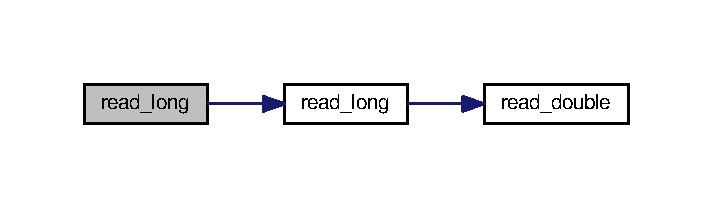
\includegraphics[width=342pt]{console__input_8h_a03ebbd2a45117ee03be4e9002210ab36_cgraph}
\end{center}
\end{figure}


\hypertarget{console__input_8h_a710a686867142de265860584f4147592}{\index{console\-\_\-input.\-h@{console\-\_\-input.\-h}!read\-\_\-long@{read\-\_\-long}}
\index{read\-\_\-long@{read\-\_\-long}!console_input.h@{console\-\_\-input.\-h}}
\subsubsection[{read\-\_\-long}]{\setlength{\rightskip}{0pt plus 5cm}long read\-\_\-long (
\begin{DoxyParamCaption}
\item[{long}]{min, }
\item[{long}]{max}
\end{DoxyParamCaption}
)}}\label{console__input_8h_a710a686867142de265860584f4147592}
Reads a long value in between a given interval from the console. When the entered value is not valid to the interval, the user gets prompted to reenter a valid.


\begin{DoxyParams}{Parameters}
{\em min} & lower bound of the interval. \\
\hline
{\em max} & top bound of the interval\\
\hline
\end{DoxyParams}
\begin{DoxyReturn}{Returns}
a long value in between min and max. 
\end{DoxyReturn}


Here is the call graph for this function\-:\nopagebreak
\begin{figure}[H]
\begin{center}
\leavevmode
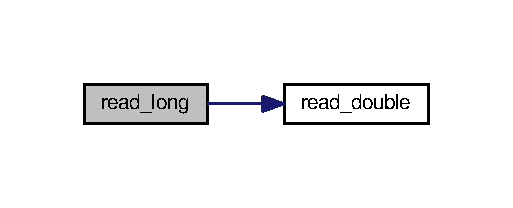
\includegraphics[width=246pt]{console__input_8h_a710a686867142de265860584f4147592_cgraph}
\end{center}
\end{figure}


\hypertarget{console__input_8h_a9128c63513d87af5259597d8c9930476}{\index{console\-\_\-input.\-h@{console\-\_\-input.\-h}!read\-\_\-long@{read\-\_\-long}}
\index{read\-\_\-long@{read\-\_\-long}!console_input.h@{console\-\_\-input.\-h}}
\subsubsection[{read\-\_\-long}]{\setlength{\rightskip}{0pt plus 5cm}long read\-\_\-long (
\begin{DoxyParamCaption}
\item[{string}]{text}
\end{DoxyParamCaption}
)}}\label{console__input_8h_a9128c63513d87af5259597d8c9930476}
Prints a text to the console and reads a long value from the console in between the whole range of long.


\begin{DoxyParams}{Parameters}
{\em text} & text to print to the console.\\
\hline
\end{DoxyParams}
\begin{DoxyReturn}{Returns}
a valid long value. 
\end{DoxyReturn}


Here is the call graph for this function\-:\nopagebreak
\begin{figure}[H]
\begin{center}
\leavevmode
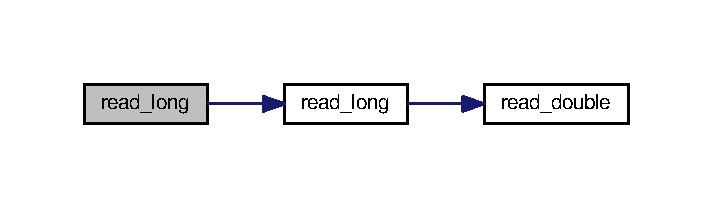
\includegraphics[width=342pt]{console__input_8h_a9128c63513d87af5259597d8c9930476_cgraph}
\end{center}
\end{figure}


\hypertarget{console__input_8h_a347c616893b725a74f60ea1f7ee325d2}{\index{console\-\_\-input.\-h@{console\-\_\-input.\-h}!read\-\_\-long@{read\-\_\-long}}
\index{read\-\_\-long@{read\-\_\-long}!console_input.h@{console\-\_\-input.\-h}}
\subsubsection[{read\-\_\-long}]{\setlength{\rightskip}{0pt plus 5cm}long read\-\_\-long (
\begin{DoxyParamCaption}
{}
\end{DoxyParamCaption}
)}}\label{console__input_8h_a347c616893b725a74f60ea1f7ee325d2}
Reads a long value from the terminal in between the whole range of long.

\begin{DoxyReturn}{Returns}
a valid long value. 
\end{DoxyReturn}


Here is the call graph for this function\-:\nopagebreak
\begin{figure}[H]
\begin{center}
\leavevmode
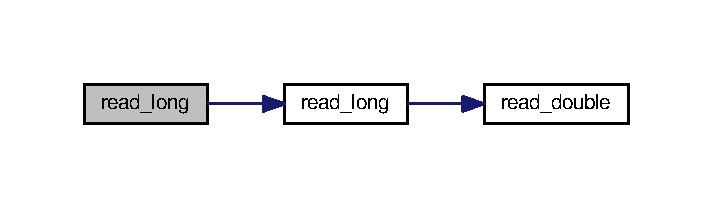
\includegraphics[width=342pt]{console__input_8h_a347c616893b725a74f60ea1f7ee325d2_cgraph}
\end{center}
\end{figure}


\hypertarget{console__input_8h_a44ccadd65be527f89bdcf6d27a3b1147}{\index{console\-\_\-input.\-h@{console\-\_\-input.\-h}!read\-\_\-text@{read\-\_\-text}}
\index{read\-\_\-text@{read\-\_\-text}!console_input.h@{console\-\_\-input.\-h}}
\subsubsection[{read\-\_\-text}]{\setlength{\rightskip}{0pt plus 5cm}string read\-\_\-text (
\begin{DoxyParamCaption}
\item[{string}]{text}
\end{DoxyParamCaption}
)}}\label{console__input_8h_a44ccadd65be527f89bdcf6d27a3b1147}
\hypertarget{console__input_8h_a6bac3909a28fff2736a171022343380b}{\index{console\-\_\-input.\-h@{console\-\_\-input.\-h}!read\-\_\-yes\-\_\-no@{read\-\_\-yes\-\_\-no}}
\index{read\-\_\-yes\-\_\-no@{read\-\_\-yes\-\_\-no}!console_input.h@{console\-\_\-input.\-h}}
\subsubsection[{read\-\_\-yes\-\_\-no}]{\setlength{\rightskip}{0pt plus 5cm}bool read\-\_\-yes\-\_\-no (
\begin{DoxyParamCaption}
\item[{string}]{text}
\end{DoxyParamCaption}
)}}\label{console__input_8h_a6bac3909a28fff2736a171022343380b}

\hypertarget{fraction_8cpp}{\section{fraction.\-cpp File Reference}
\label{fraction_8cpp}\index{fraction.\-cpp@{fraction.\-cpp}}
}
{\ttfamily \#include $<$sstream$>$}\\*
{\ttfamily \#include $<$iostream$>$}\\*
{\ttfamily \#include $<$ctime$>$}\\*
{\ttfamily \#include $<$cstdlib$>$}\\*
{\ttfamily \#include $<$stdexcept$>$}\\*
{\ttfamily \#include \char`\"{}console\-\_\-input.\-h\char`\"{}}\\*
{\ttfamily \#include \char`\"{}fraction.\-h\char`\"{}}\\*
Include dependency graph for fraction.\-cpp\-:\nopagebreak
\begin{figure}[H]
\begin{center}
\leavevmode
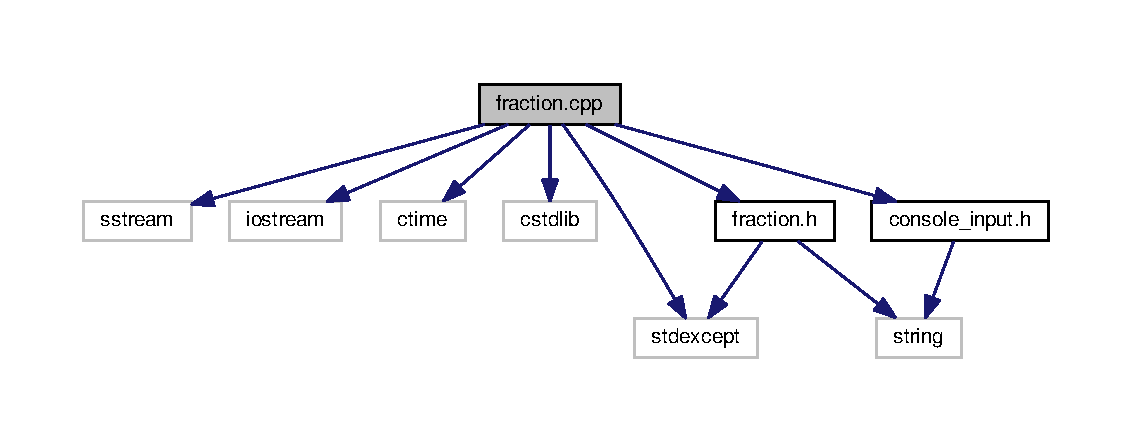
\includegraphics[width=350pt]{fraction_8cpp__incl}
\end{center}
\end{figure}
\subsection*{Functions}
\begin{DoxyCompactItemize}
\item 
\hyperlink{classFraction}{Fraction} \hyperlink{fraction_8cpp_a01030474607789a59c23832eaa96afcd}{operator+} (const int \&left, const \hyperlink{classFraction}{Fraction} \&right)
\item 
\hyperlink{classFraction}{Fraction} \hyperlink{fraction_8cpp_aeef49237f5f33865b83ed6a335225392}{operator-\/} (const int \&left, const \hyperlink{classFraction}{Fraction} \&right)
\item 
\hyperlink{classFraction}{Fraction} \hyperlink{fraction_8cpp_a9ebcb6c3e3ca935833b8a5b69ca9e9a2}{operator$\ast$} (const int \&left, const \hyperlink{classFraction}{Fraction} \&right)
\item 
\hyperlink{classFraction}{Fraction} \hyperlink{fraction_8cpp_acd5918eb57ec3a95dcfb402f486e4ff3}{operator/} (const int \&left, const \hyperlink{classFraction}{Fraction} \&right)
\item 
istream \& \hyperlink{fraction_8cpp_aa459309e7314753308bc9d1cde5bbb9e}{operator$>$$>$} (istream \&input, \hyperlink{classFraction}{Fraction} \&frc)
\item 
std\-::ostream \& \hyperlink{fraction_8cpp_a6bbb30df04fbf0667ea707be92ee40ae}{operator$<$$<$} (std\-::ostream \&output, const \hyperlink{classFraction}{Fraction} \&frc)
\end{DoxyCompactItemize}


\subsection{Function Documentation}
\hypertarget{fraction_8cpp_a9ebcb6c3e3ca935833b8a5b69ca9e9a2}{\index{fraction.\-cpp@{fraction.\-cpp}!operator$\ast$@{operator$\ast$}}
\index{operator$\ast$@{operator$\ast$}!fraction.cpp@{fraction.\-cpp}}
\subsubsection[{operator$\ast$}]{\setlength{\rightskip}{0pt plus 5cm}{\bf Fraction} operator$\ast$ (
\begin{DoxyParamCaption}
\item[{const int \&}]{left, }
\item[{const {\bf Fraction} \&}]{right}
\end{DoxyParamCaption}
)}}\label{fraction_8cpp_a9ebcb6c3e3ca935833b8a5b69ca9e9a2}
Overloads the global operator$\ast$. Defines how to multiply an Integer and a \hyperlink{classFraction}{Fraction} and returns the multiplication as a new \hyperlink{classFraction}{Fraction}.


\begin{DoxyParams}{Parameters}
{\em left} & Integer as multiplicator \\
\hline
{\em right} & \hyperlink{classFraction}{Fraction} as multiplicator\\
\hline
\end{DoxyParams}
\begin{DoxyReturn}{Returns}
a \hyperlink{classFraction}{Fraction} with the multiplication of the integer and \hyperlink{classFraction}{Fraction}. 
\end{DoxyReturn}
\hypertarget{fraction_8cpp_a01030474607789a59c23832eaa96afcd}{\index{fraction.\-cpp@{fraction.\-cpp}!operator+@{operator+}}
\index{operator+@{operator+}!fraction.cpp@{fraction.\-cpp}}
\subsubsection[{operator+}]{\setlength{\rightskip}{0pt plus 5cm}{\bf Fraction} operator+ (
\begin{DoxyParamCaption}
\item[{const int \&}]{left, }
\item[{const {\bf Fraction} \&}]{right}
\end{DoxyParamCaption}
)}}\label{fraction_8cpp_a01030474607789a59c23832eaa96afcd}
Overloads global operatr+. Defines how to add a \hyperlink{classFraction}{Fraction} to an integer and returns the sum as a new \hyperlink{classFraction}{Fraction}.


\begin{DoxyParams}{Parameters}
{\em left} & Integer to which the \hyperlink{classFraction}{Fraction} gets added. \\
\hline
{\em right} & \hyperlink{classFraction}{Fraction} which gets added.\\
\hline
\end{DoxyParams}
\begin{DoxyReturn}{Returns}
a \hyperlink{classFraction}{Fraction} with the sum of the integer and \hyperlink{classFraction}{Fraction}. 
\end{DoxyReturn}
\hypertarget{fraction_8cpp_aeef49237f5f33865b83ed6a335225392}{\index{fraction.\-cpp@{fraction.\-cpp}!operator-\/@{operator-\/}}
\index{operator-\/@{operator-\/}!fraction.cpp@{fraction.\-cpp}}
\subsubsection[{operator-\/}]{\setlength{\rightskip}{0pt plus 5cm}{\bf Fraction} operator-\/ (
\begin{DoxyParamCaption}
\item[{const int \&}]{left, }
\item[{const {\bf Fraction} \&}]{right}
\end{DoxyParamCaption}
)}}\label{fraction_8cpp_aeef49237f5f33865b83ed6a335225392}
Overloads the global operator-\/. Defines how to subtract a \hyperlink{classFraction}{Fraction} from an integer and returns the difference as a new \hyperlink{classFraction}{Fraction}.


\begin{DoxyParams}{Parameters}
{\em left} & Integer from which the \hyperlink{classFraction}{Fraction} gets subtracted. \\
\hline
{\em right} & \hyperlink{classFraction}{Fraction} to subtract from the Integer.\\
\hline
\end{DoxyParams}
\begin{DoxyReturn}{Returns}
a \hyperlink{classFraction}{Fraction} with the sum of the integer and \hyperlink{classFraction}{Fraction}. 
\end{DoxyReturn}
\hypertarget{fraction_8cpp_acd5918eb57ec3a95dcfb402f486e4ff3}{\index{fraction.\-cpp@{fraction.\-cpp}!operator/@{operator/}}
\index{operator/@{operator/}!fraction.cpp@{fraction.\-cpp}}
\subsubsection[{operator/}]{\setlength{\rightskip}{0pt plus 5cm}{\bf Fraction} operator/ (
\begin{DoxyParamCaption}
\item[{const int \&}]{left, }
\item[{const {\bf Fraction} \&}]{right}
\end{DoxyParamCaption}
)}}\label{fraction_8cpp_acd5918eb57ec3a95dcfb402f486e4ff3}
Overloads the global operator/. Defines how to divide an Integer by a \hyperlink{classFraction}{Fraction} and returns the division as a new \hyperlink{classFraction}{Fraction}.


\begin{DoxyParams}{Parameters}
{\em left} & Integer as numerator. \\
\hline
{\em right} & \hyperlink{classFraction}{Fraction} as denumerator.\\
\hline
\end{DoxyParams}
\begin{DoxyReturn}{Returns}
a \hyperlink{classFraction}{Fraction} with the division of the integer by the \hyperlink{classFraction}{Fraction}. 
\end{DoxyReturn}
\hypertarget{fraction_8cpp_a6bbb30df04fbf0667ea707be92ee40ae}{\index{fraction.\-cpp@{fraction.\-cpp}!operator$<$$<$@{operator$<$$<$}}
\index{operator$<$$<$@{operator$<$$<$}!fraction.cpp@{fraction.\-cpp}}
\subsubsection[{operator$<$$<$}]{\setlength{\rightskip}{0pt plus 5cm}std\-::ostream\& operator$<$$<$ (
\begin{DoxyParamCaption}
\item[{std\-::ostream \&}]{output, }
\item[{const {\bf Fraction} \&}]{frc}
\end{DoxyParamCaption}
)}}\label{fraction_8cpp_a6bbb30df04fbf0667ea707be92ee40ae}
Overloads the global operator$<$$<$ \char`\"{}put to\char`\"{}. Defines how a \hyperlink{classFraction}{Fraction} gets printed out to the outputstream.

Format\-: numerator/denominator 1/1, 0/3, 89/2, -\/9/7


\begin{DoxyParams}{Parameters}
{\em output} & Outputstream. \\
\hline
{\em frc} & \hyperlink{classFraction}{Fraction} to print to the outputstream.\\
\hline
\end{DoxyParams}
\begin{DoxyReturn}{Returns}
the given outputstream output. 
\end{DoxyReturn}


Here is the call graph for this function\-:\nopagebreak
\begin{figure}[H]
\begin{center}
\leavevmode
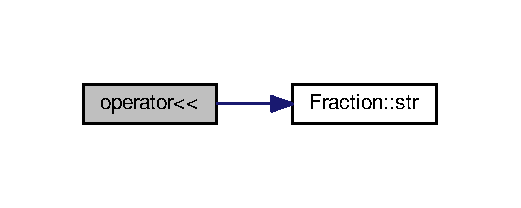
\includegraphics[width=250pt]{fraction_8cpp_a6bbb30df04fbf0667ea707be92ee40ae_cgraph}
\end{center}
\end{figure}


\hypertarget{fraction_8cpp_aa459309e7314753308bc9d1cde5bbb9e}{\index{fraction.\-cpp@{fraction.\-cpp}!operator$>$$>$@{operator$>$$>$}}
\index{operator$>$$>$@{operator$>$$>$}!fraction.cpp@{fraction.\-cpp}}
\subsubsection[{operator$>$$>$}]{\setlength{\rightskip}{0pt plus 5cm}istream\& operator$>$$>$ (
\begin{DoxyParamCaption}
\item[{istream \&}]{input, }
\item[{{\bf Fraction} \&}]{frc}
\end{DoxyParamCaption}
)}}\label{fraction_8cpp_aa459309e7314753308bc9d1cde5bbb9e}
Overloads the global operator$>$$>$ \char`\"{}get from\char`\"{}. Defines the entry of a fraction from the user by the console.


\begin{DoxyParams}{Parameters}
{\em input} & Input Stream. \\
\hline
{\em frc} & \hyperlink{classFraction}{Fraction} to save the userinput into.\\
\hline
\end{DoxyParams}
\begin{DoxyReturn}{Returns}
the given inputstream input. 
\end{DoxyReturn}


Here is the call graph for this function\-:\nopagebreak
\begin{figure}[H]
\begin{center}
\leavevmode
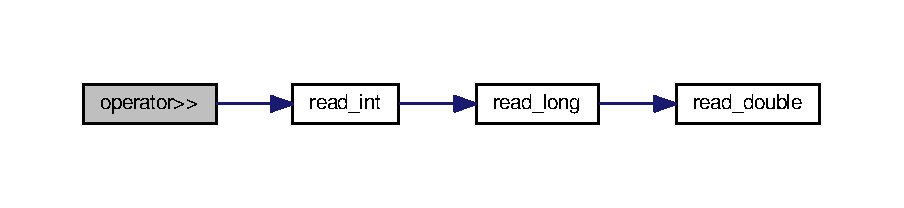
\includegraphics[width=350pt]{fraction_8cpp_aa459309e7314753308bc9d1cde5bbb9e_cgraph}
\end{center}
\end{figure}



\hypertarget{fraction_8h}{\section{fraction.\-h File Reference}
\label{fraction_8h}\index{fraction.\-h@{fraction.\-h}}
}
{\ttfamily \#include $<$string$>$}\\*
{\ttfamily \#include $<$stdexcept$>$}\\*
Include dependency graph for fraction.\-h\-:\nopagebreak
\begin{figure}[H]
\begin{center}
\leavevmode
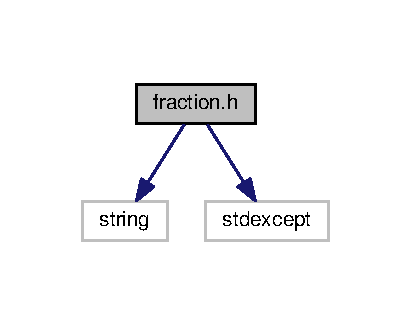
\includegraphics[width=197pt]{fraction_8h__incl}
\end{center}
\end{figure}
This graph shows which files directly or indirectly include this file\-:\nopagebreak
\begin{figure}[H]
\begin{center}
\leavevmode
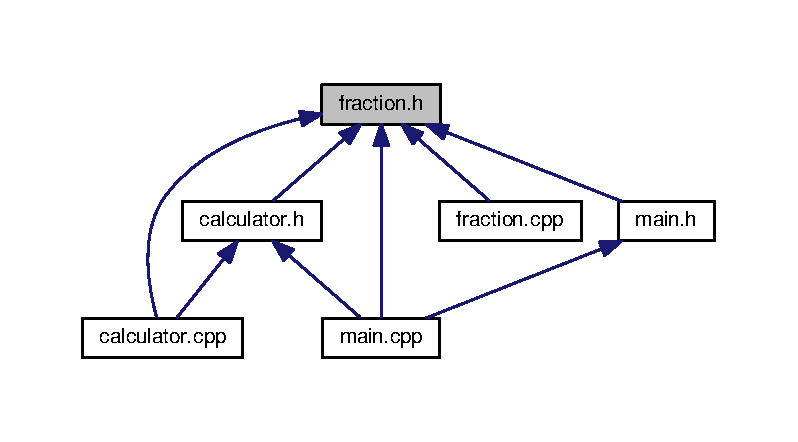
\includegraphics[width=350pt]{fraction_8h__dep__incl}
\end{center}
\end{figure}
\subsection*{Classes}
\begin{DoxyCompactItemize}
\item 
class \hyperlink{classFraction}{Fraction}
\end{DoxyCompactItemize}
\subsection*{Functions}
\begin{DoxyCompactItemize}
\item 
\hyperlink{classFraction}{Fraction} \hyperlink{fraction_8h_a01030474607789a59c23832eaa96afcd}{operator+} (const int \&left, const \hyperlink{classFraction}{Fraction} \&right)
\item 
\hyperlink{classFraction}{Fraction} \hyperlink{fraction_8h_aeef49237f5f33865b83ed6a335225392}{operator-\/} (const int \&left, const \hyperlink{classFraction}{Fraction} \&right)
\item 
\hyperlink{classFraction}{Fraction} \hyperlink{fraction_8h_a9ebcb6c3e3ca935833b8a5b69ca9e9a2}{operator$\ast$} (const int \&left, const \hyperlink{classFraction}{Fraction} \&right)
\item 
\hyperlink{classFraction}{Fraction} \hyperlink{fraction_8h_acd5918eb57ec3a95dcfb402f486e4ff3}{operator/} (const int \&left, const \hyperlink{classFraction}{Fraction} \&right)
\item 
std\-::istream \& \hyperlink{fraction_8h_af910e291818debfe7e7a3ef08c05b81c}{operator$>$$>$} (std\-::istream \&input, \hyperlink{classFraction}{Fraction} \&right)
\item 
std\-::ostream \& \hyperlink{fraction_8h_a6bbb30df04fbf0667ea707be92ee40ae}{operator$<$$<$} (std\-::ostream \&output, const \hyperlink{classFraction}{Fraction} \&frc)
\end{DoxyCompactItemize}


\subsection{Function Documentation}
\hypertarget{fraction_8h_a9ebcb6c3e3ca935833b8a5b69ca9e9a2}{\index{fraction.\-h@{fraction.\-h}!operator$\ast$@{operator$\ast$}}
\index{operator$\ast$@{operator$\ast$}!fraction.h@{fraction.\-h}}
\subsubsection[{operator$\ast$}]{\setlength{\rightskip}{0pt plus 5cm}{\bf Fraction} operator$\ast$ (
\begin{DoxyParamCaption}
\item[{const int \&}]{left, }
\item[{const {\bf Fraction} \&}]{right}
\end{DoxyParamCaption}
)}}\label{fraction_8h_a9ebcb6c3e3ca935833b8a5b69ca9e9a2}
Overloads the global operator$\ast$. Defines how to multiply an Integer and a \hyperlink{classFraction}{Fraction} and returns the multiplication as a new \hyperlink{classFraction}{Fraction}.


\begin{DoxyParams}{Parameters}
{\em left} & Integer as multiplicator \\
\hline
{\em right} & \hyperlink{classFraction}{Fraction} as multiplicator\\
\hline
\end{DoxyParams}
\begin{DoxyReturn}{Returns}
a \hyperlink{classFraction}{Fraction} with the multiplication of the integer and \hyperlink{classFraction}{Fraction}. 
\end{DoxyReturn}
\hypertarget{fraction_8h_a01030474607789a59c23832eaa96afcd}{\index{fraction.\-h@{fraction.\-h}!operator+@{operator+}}
\index{operator+@{operator+}!fraction.h@{fraction.\-h}}
\subsubsection[{operator+}]{\setlength{\rightskip}{0pt plus 5cm}{\bf Fraction} operator+ (
\begin{DoxyParamCaption}
\item[{const int \&}]{left, }
\item[{const {\bf Fraction} \&}]{right}
\end{DoxyParamCaption}
)}}\label{fraction_8h_a01030474607789a59c23832eaa96afcd}
Overloads global operatr+. Defines how to add a \hyperlink{classFraction}{Fraction} to an integer and returns the sum as a new \hyperlink{classFraction}{Fraction}.


\begin{DoxyParams}{Parameters}
{\em left} & Integer to which the \hyperlink{classFraction}{Fraction} gets added. \\
\hline
{\em right} & \hyperlink{classFraction}{Fraction} which gets added.\\
\hline
\end{DoxyParams}
\begin{DoxyReturn}{Returns}
a \hyperlink{classFraction}{Fraction} with the sum of the integer and \hyperlink{classFraction}{Fraction}. 
\end{DoxyReturn}
\hypertarget{fraction_8h_aeef49237f5f33865b83ed6a335225392}{\index{fraction.\-h@{fraction.\-h}!operator-\/@{operator-\/}}
\index{operator-\/@{operator-\/}!fraction.h@{fraction.\-h}}
\subsubsection[{operator-\/}]{\setlength{\rightskip}{0pt plus 5cm}{\bf Fraction} operator-\/ (
\begin{DoxyParamCaption}
\item[{const int \&}]{left, }
\item[{const {\bf Fraction} \&}]{right}
\end{DoxyParamCaption}
)}}\label{fraction_8h_aeef49237f5f33865b83ed6a335225392}
Overloads the global operator-\/. Defines how to subtract a \hyperlink{classFraction}{Fraction} from an integer and returns the difference as a new \hyperlink{classFraction}{Fraction}.


\begin{DoxyParams}{Parameters}
{\em left} & Integer from which the \hyperlink{classFraction}{Fraction} gets subtracted. \\
\hline
{\em right} & \hyperlink{classFraction}{Fraction} to subtract from the Integer.\\
\hline
\end{DoxyParams}
\begin{DoxyReturn}{Returns}
a \hyperlink{classFraction}{Fraction} with the sum of the integer and \hyperlink{classFraction}{Fraction}. 
\end{DoxyReturn}
\hypertarget{fraction_8h_acd5918eb57ec3a95dcfb402f486e4ff3}{\index{fraction.\-h@{fraction.\-h}!operator/@{operator/}}
\index{operator/@{operator/}!fraction.h@{fraction.\-h}}
\subsubsection[{operator/}]{\setlength{\rightskip}{0pt plus 5cm}{\bf Fraction} operator/ (
\begin{DoxyParamCaption}
\item[{const int \&}]{left, }
\item[{const {\bf Fraction} \&}]{right}
\end{DoxyParamCaption}
)}}\label{fraction_8h_acd5918eb57ec3a95dcfb402f486e4ff3}
Overloads the global operator/. Defines how to divide an Integer by a \hyperlink{classFraction}{Fraction} and returns the division as a new \hyperlink{classFraction}{Fraction}.


\begin{DoxyParams}{Parameters}
{\em left} & Integer as numerator. \\
\hline
{\em right} & \hyperlink{classFraction}{Fraction} as denumerator.\\
\hline
\end{DoxyParams}
\begin{DoxyReturn}{Returns}
a \hyperlink{classFraction}{Fraction} with the division of the integer by the \hyperlink{classFraction}{Fraction}. 
\end{DoxyReturn}
\hypertarget{fraction_8h_a6bbb30df04fbf0667ea707be92ee40ae}{\index{fraction.\-h@{fraction.\-h}!operator$<$$<$@{operator$<$$<$}}
\index{operator$<$$<$@{operator$<$$<$}!fraction.h@{fraction.\-h}}
\subsubsection[{operator$<$$<$}]{\setlength{\rightskip}{0pt plus 5cm}std\-::ostream\& operator$<$$<$ (
\begin{DoxyParamCaption}
\item[{std\-::ostream \&}]{output, }
\item[{const {\bf Fraction} \&}]{frc}
\end{DoxyParamCaption}
)}}\label{fraction_8h_a6bbb30df04fbf0667ea707be92ee40ae}
Overloads the global operator$<$$<$ \char`\"{}put to\char`\"{}. Defines how a \hyperlink{classFraction}{Fraction} gets printed out to the outputstream.

Format\-: numerator/denominator 1/1, 0/3, 89/2, -\/9/7


\begin{DoxyParams}{Parameters}
{\em output} & Outputstream. \\
\hline
{\em frc} & \hyperlink{classFraction}{Fraction} to print to the outputstream.\\
\hline
\end{DoxyParams}
\begin{DoxyReturn}{Returns}
the given outputstream output. 
\end{DoxyReturn}


Here is the call graph for this function\-:\nopagebreak
\begin{figure}[H]
\begin{center}
\leavevmode
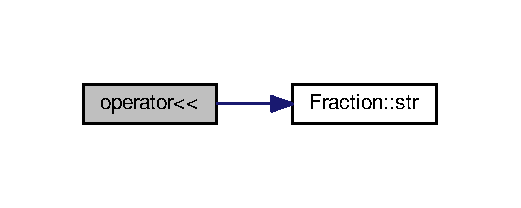
\includegraphics[width=250pt]{fraction_8h_a6bbb30df04fbf0667ea707be92ee40ae_cgraph}
\end{center}
\end{figure}


\hypertarget{fraction_8h_af910e291818debfe7e7a3ef08c05b81c}{\index{fraction.\-h@{fraction.\-h}!operator$>$$>$@{operator$>$$>$}}
\index{operator$>$$>$@{operator$>$$>$}!fraction.h@{fraction.\-h}}
\subsubsection[{operator$>$$>$}]{\setlength{\rightskip}{0pt plus 5cm}std\-::istream\& operator$>$$>$ (
\begin{DoxyParamCaption}
\item[{std\-::istream \&}]{input, }
\item[{{\bf Fraction} \&}]{right}
\end{DoxyParamCaption}
)}}\label{fraction_8h_af910e291818debfe7e7a3ef08c05b81c}

\hypertarget{fraction__main_8cpp}{\section{fraction\-\_\-main.\-cpp File Reference}
\label{fraction__main_8cpp}\index{fraction\-\_\-main.\-cpp@{fraction\-\_\-main.\-cpp}}
}
{\ttfamily \#include $<$iostream$>$}\\*
{\ttfamily \#include $<$iomanip$>$}\\*
{\ttfamily \#include $<$string.\-h$>$}\\*
{\ttfamily \#include $<$sstream$>$}\\*
{\ttfamily \#include $<$fstream$>$}\\*
{\ttfamily \#include $<$cstdlib$>$}\\*
{\ttfamily \#include $<$vector$>$}\\*
{\ttfamily \#include $<$stdexcept$>$}\\*
{\ttfamily \#include \char`\"{}fraction\-\_\-main.\-h\char`\"{}}\\*
{\ttfamily \#include \char`\"{}fraction.\-h\char`\"{}}\\*
{\ttfamily \#include \char`\"{}calculator.\-h\char`\"{}}\\*
Include dependency graph for fraction\-\_\-main.\-cpp\-:\nopagebreak
\begin{figure}[H]
\begin{center}
\leavevmode
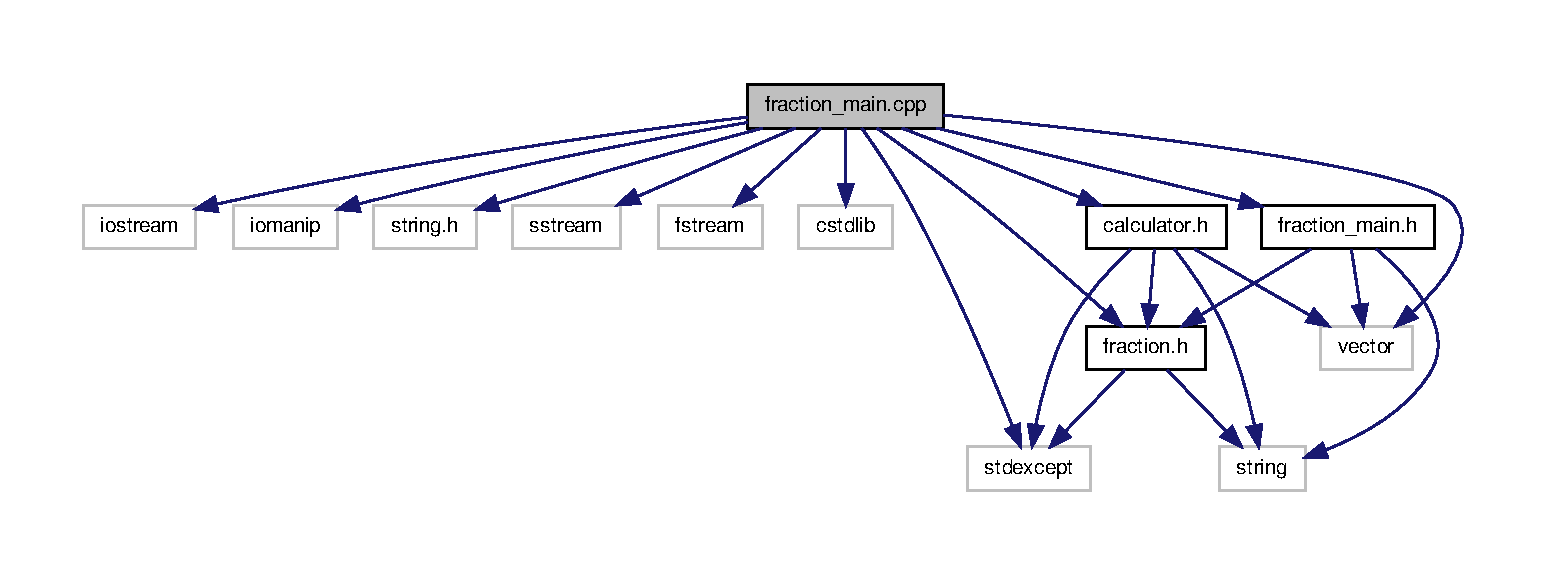
\includegraphics[width=350pt]{fraction__main_8cpp__incl}
\end{center}
\end{figure}
\subsection*{Functions}
\begin{DoxyCompactItemize}
\item 
int \hyperlink{fraction__main_8cpp_a0ddf1224851353fc92bfbff6f499fa97}{main} (int argc, char $\ast$argv\mbox{[}$\,$\mbox{]})
\item 
void \hyperlink{fraction__main_8cpp_a88a5a1f559a0f664dbb99b66f6c86c59}{handle\-\_\-five} (char $\ast$argv\mbox{[}$\,$\mbox{]})
\item 
void \hyperlink{fraction__main_8cpp_afbc888f515c7c31845c525098c70a949}{handle\-\_\-six} (char $\ast$argv\mbox{[}$\,$\mbox{]})
\item 
void \hyperlink{fraction__main_8cpp_a6d598685a1aa70dc69dc3d66f694415d}{handle\-\_\-nine} (char $\ast$argv\mbox{[}$\,$\mbox{]})
\item 
bool \hyperlink{fraction__main_8cpp_a1920cd03342937f72cb6c49041a6953d}{isi} (char text\mbox{[}$\,$\mbox{]})
\item 
void \hyperlink{fraction__main_8cpp_a45ba46a5ae34b55a833eced785f695ea}{random\-\_\-handler} (int n, int a, int b, int c, int d, bool asc)
\item 
std\-::vector$<$ \hyperlink{classFraction}{Fraction} $>$ \hyperlink{fraction__main_8cpp_a75b94fb0a8fdbf6d97e5cf1f55997549}{random\-\_\-fractions} (int n, int low\-\_\-numerator, int low\-\_\-denominator, int high\-\_\-numerator, int high\-\_\-denominator)  throw (const std\-::invalid\-\_\-argument)
\item 
void \hyperlink{fraction__main_8cpp_a5703c295722633fe65e49e83e620c6b5}{sort} (std\-::vector$<$ \hyperlink{classFraction}{Fraction} $>$ \&fractions, int length, bool asc)
\item 
void \hyperlink{fraction__main_8cpp_a7c827c26e5661b0c05da029a209d0cb8}{show\-\_\-manual} ()
\end{DoxyCompactItemize}


\subsection{Function Documentation}
\hypertarget{fraction__main_8cpp_a88a5a1f559a0f664dbb99b66f6c86c59}{\index{fraction\-\_\-main.\-cpp@{fraction\-\_\-main.\-cpp}!handle\-\_\-five@{handle\-\_\-five}}
\index{handle\-\_\-five@{handle\-\_\-five}!fraction_main.cpp@{fraction\-\_\-main.\-cpp}}
\subsubsection[{handle\-\_\-five}]{\setlength{\rightskip}{0pt plus 5cm}void handle\-\_\-five (
\begin{DoxyParamCaption}
\item[{char $\ast$}]{argv\mbox{[}$\,$\mbox{]}}
\end{DoxyParamCaption}
)}}\label{fraction__main_8cpp_a88a5a1f559a0f664dbb99b66f6c86c59}
Handles program when executed with five arguments. Validates input format.

Possible actions are\-: bruch a op c d a op c/d = e/f =$>$ bruch 1 -\/ 1 2 1 -\/ 1/2 = 1/2 bruch a b op c a/b op c = e/f =$>$ bruch 1 2 -\/ 1 1/2 -\/ 1 = -\/1/2


\begin{DoxyParams}{Parameters}
{\em $\ast$argv\mbox{[}$\,$\mbox{]}} & Arguments array form the program execution. \\
\hline
\end{DoxyParams}


Here is the call graph for this function\-:\nopagebreak
\begin{figure}[H]
\begin{center}
\leavevmode
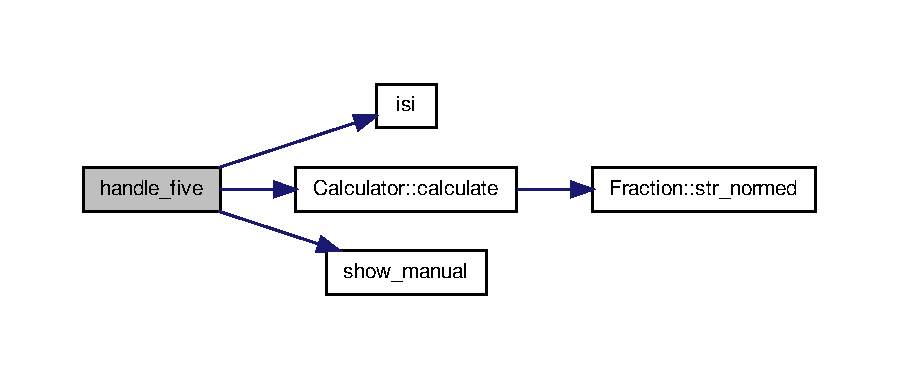
\includegraphics[width=350pt]{fraction__main_8cpp_a88a5a1f559a0f664dbb99b66f6c86c59_cgraph}
\end{center}
\end{figure}


\hypertarget{fraction__main_8cpp_a6d598685a1aa70dc69dc3d66f694415d}{\index{fraction\-\_\-main.\-cpp@{fraction\-\_\-main.\-cpp}!handle\-\_\-nine@{handle\-\_\-nine}}
\index{handle\-\_\-nine@{handle\-\_\-nine}!fraction_main.cpp@{fraction\-\_\-main.\-cpp}}
\subsubsection[{handle\-\_\-nine}]{\setlength{\rightskip}{0pt plus 5cm}void handle\-\_\-nine (
\begin{DoxyParamCaption}
\item[{char $\ast$}]{argv\mbox{[}$\,$\mbox{]}}
\end{DoxyParamCaption}
)}}\label{fraction__main_8cpp_a6d598685a1aa70dc69dc3d66f694415d}
Handles program when executed with nine arguments. Validates input format.

Possible actions are\-: bruch n \mbox{[} a b c d \mbox{]} + n numbers between a/b and c/d ascendent sorted. bruch n \mbox{[} a b c d \mbox{]} -\/ n numbers between a/b and c/d descendent sorted.


\begin{DoxyParams}{Parameters}
{\em $\ast$argv\mbox{[}$\,$\mbox{]}} & Arguments array form the program execution. \\
\hline
\end{DoxyParams}


Here is the call graph for this function\-:\nopagebreak
\begin{figure}[H]
\begin{center}
\leavevmode
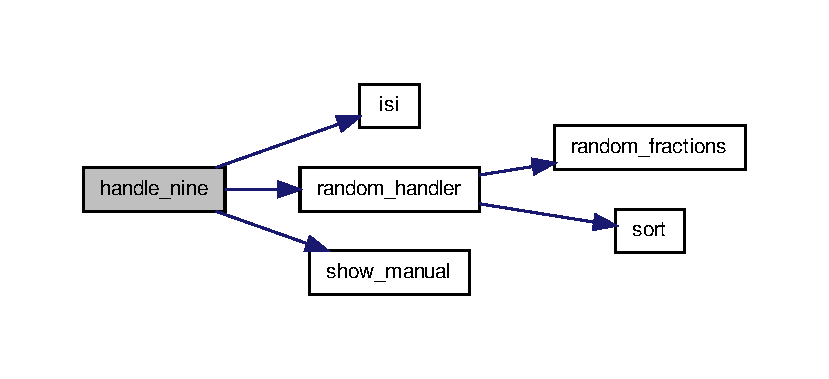
\includegraphics[width=350pt]{fraction__main_8cpp_a6d598685a1aa70dc69dc3d66f694415d_cgraph}
\end{center}
\end{figure}


\hypertarget{fraction__main_8cpp_afbc888f515c7c31845c525098c70a949}{\index{fraction\-\_\-main.\-cpp@{fraction\-\_\-main.\-cpp}!handle\-\_\-six@{handle\-\_\-six}}
\index{handle\-\_\-six@{handle\-\_\-six}!fraction_main.cpp@{fraction\-\_\-main.\-cpp}}
\subsubsection[{handle\-\_\-six}]{\setlength{\rightskip}{0pt plus 5cm}void handle\-\_\-six (
\begin{DoxyParamCaption}
\item[{char $\ast$}]{argv\mbox{[}$\,$\mbox{]}}
\end{DoxyParamCaption}
)}}\label{fraction__main_8cpp_afbc888f515c7c31845c525098c70a949}
Handles program when executed with six arguments. Validates input format.

Possible actions are\-: bruch a b op c d a/b op c/d = e/f =$>$ bruch 1 2 -\/ 1 3 1/2 -\/ 1/3 = 1/6 bruch a b -\/v c d a/b \mbox{[}$<$$|$$>$$|$=\mbox{]} c/d =$>$ 1 2 -\/v 1 3 1/2 $>$ 1/3


\begin{DoxyParams}{Parameters}
{\em $\ast$argv\mbox{[}$\,$\mbox{]}} & Arguments array form the program execution. \\
\hline
\end{DoxyParams}


Here is the call graph for this function\-:\nopagebreak
\begin{figure}[H]
\begin{center}
\leavevmode
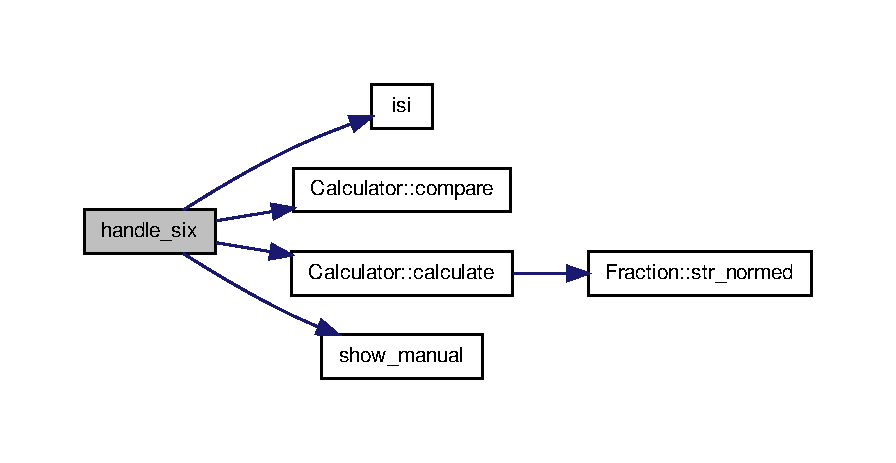
\includegraphics[width=350pt]{fraction__main_8cpp_afbc888f515c7c31845c525098c70a949_cgraph}
\end{center}
\end{figure}


\hypertarget{fraction__main_8cpp_a1920cd03342937f72cb6c49041a6953d}{\index{fraction\-\_\-main.\-cpp@{fraction\-\_\-main.\-cpp}!isi@{isi}}
\index{isi@{isi}!fraction_main.cpp@{fraction\-\_\-main.\-cpp}}
\subsubsection[{isi}]{\setlength{\rightskip}{0pt plus 5cm}bool isi (
\begin{DoxyParamCaption}
\item[{char}]{text\mbox{[}$\,$\mbox{]}}
\end{DoxyParamCaption}
)}}\label{fraction__main_8cpp_a1920cd03342937f72cb6c49041a6953d}
Checks whether an array of chars represents an integer or not. Solfs atoi problem that returns a 0 for a char which is not a number.


\begin{DoxyParams}{Parameters}
{\em text\mbox{[}$\,$\mbox{]}} & Array of chars.\\
\hline
\end{DoxyParams}
\begin{DoxyReturn}{Returns}
true when text\mbox{[}\mbox{]} represents a number. false when text\mbox{[}\mbox{]} doesn't represent a number. 
\end{DoxyReturn}
\hypertarget{fraction__main_8cpp_a0ddf1224851353fc92bfbff6f499fa97}{\index{fraction\-\_\-main.\-cpp@{fraction\-\_\-main.\-cpp}!main@{main}}
\index{main@{main}!fraction_main.cpp@{fraction\-\_\-main.\-cpp}}
\subsubsection[{main}]{\setlength{\rightskip}{0pt plus 5cm}int main (
\begin{DoxyParamCaption}
\item[{int}]{argc, }
\item[{char $\ast$}]{argv\mbox{[}$\,$\mbox{]}}
\end{DoxyParamCaption}
)}}\label{fraction__main_8cpp_a0ddf1224851353fc92bfbff6f499fa97}
Entrypoint to the program \char`\"{}\-Bruch\char`\"{}. Bruch lets you calculate and compare Fractions directly in the console. There is also the possibility to generate random \hyperlink{classFraction}{Fraction} in a certain range. It prompts the user while inserting wrong Fractions where the denominator is zero.

Possible calculation execution forms (op = +,-\/,$\ast$,/)\-: bruch a b op c d a/b op c/d = e/f =$>$ bruch 1 2 -\/ 1 3 1/2 -\/ 1/3 = 1/6 bruch a op c d a op c/d = e/f =$>$ bruch 1 -\/ 1 2 1 -\/ 1/2 = 1/2 bruch a b op c a/b op c = e/f =$>$ bruch 1 2 -\/ 1 1/2 -\/ 1 = -\/1/2

Possible compare executions\-: bruch a b -\/v c d a/b \mbox{[}$<$$|$$>$$|$=\mbox{]} c/d =$>$ 1 2 -\/v 1 3 1/2 $>$ 1/3

Possible random number generator bruch n \mbox{[} a b c d \mbox{]} + n numbers between a/b and c/d ascendent sorted. bruch n \mbox{[} a b c d \mbox{]} -\/ n numbers between a/b and c/d descendent sorted.


\begin{DoxyParams}{Parameters}
{\em argc} & Length of the arguments array. \\
\hline
{\em $\ast$argv\mbox{[}$\,$\mbox{]}} & Arguments array form the program execution. \\
\hline
\end{DoxyParams}


Here is the call graph for this function\-:\nopagebreak
\begin{figure}[H]
\begin{center}
\leavevmode
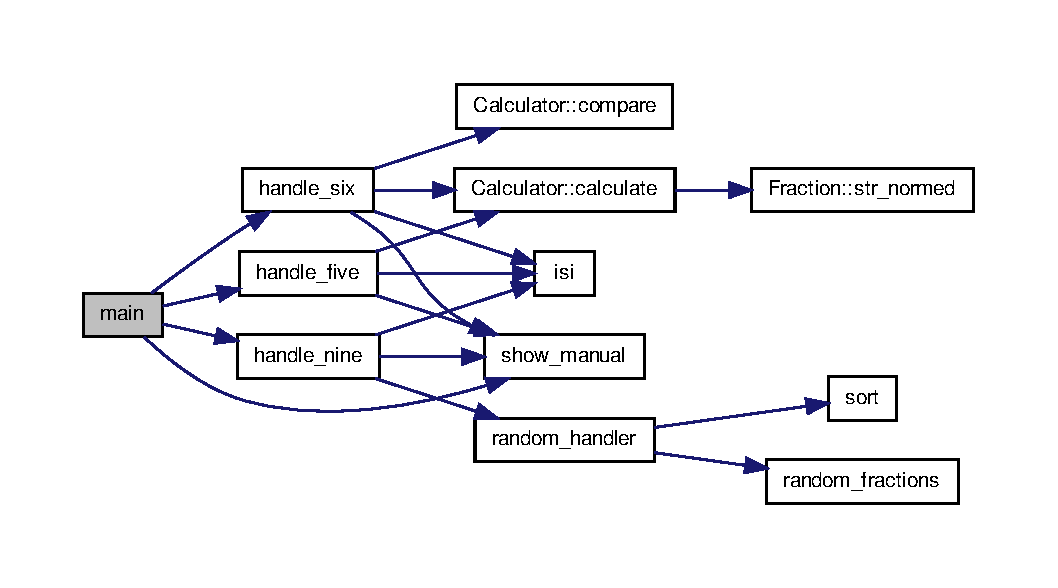
\includegraphics[width=350pt]{fraction__main_8cpp_a0ddf1224851353fc92bfbff6f499fa97_cgraph}
\end{center}
\end{figure}


\hypertarget{fraction__main_8cpp_a75b94fb0a8fdbf6d97e5cf1f55997549}{\index{fraction\-\_\-main.\-cpp@{fraction\-\_\-main.\-cpp}!random\-\_\-fractions@{random\-\_\-fractions}}
\index{random\-\_\-fractions@{random\-\_\-fractions}!fraction_main.cpp@{fraction\-\_\-main.\-cpp}}
\subsubsection[{random\-\_\-fractions}]{\setlength{\rightskip}{0pt plus 5cm}std\-::vector$<${\bf Fraction}$>$ random\-\_\-fractions (
\begin{DoxyParamCaption}
\item[{int}]{n, }
\item[{int}]{low\-\_\-numerator, }
\item[{int}]{low\-\_\-denominator, }
\item[{int}]{high\-\_\-numerator, }
\item[{int}]{high\-\_\-denominator}
\end{DoxyParamCaption}
)  throw (const std\-::invalid\-\_\-argument)}}\label{fraction__main_8cpp_a75b94fb0a8fdbf6d97e5cf1f55997549}
Generates n random Fractions with value in between the Fractions a/b and c/d and gives them back as vector.


\begin{DoxyParams}{Parameters}
{\em n} & Number of random fractions. \\
\hline
{\em low\-\_\-numerator} & Numerator of the low bound fraction. \\
\hline
{\em low\-\_\-denominator} & Denominator of the low bound fraction. \\
\hline
{\em high\-\_\-numerator} & Numerator of the high bound fraction. \\
\hline
{\em high\-\_\-denominator} & Denominator of the high bound fraction.\\
\hline
\end{DoxyParams}
\begin{DoxyReturn}{Returns}
vector with the fractions. 
\end{DoxyReturn}
\hypertarget{fraction__main_8cpp_a45ba46a5ae34b55a833eced785f695ea}{\index{fraction\-\_\-main.\-cpp@{fraction\-\_\-main.\-cpp}!random\-\_\-handler@{random\-\_\-handler}}
\index{random\-\_\-handler@{random\-\_\-handler}!fraction_main.cpp@{fraction\-\_\-main.\-cpp}}
\subsubsection[{random\-\_\-handler}]{\setlength{\rightskip}{0pt plus 5cm}void random\-\_\-handler (
\begin{DoxyParamCaption}
\item[{int}]{n, }
\item[{int}]{a, }
\item[{int}]{b, }
\item[{int}]{c, }
\item[{int}]{d, }
\item[{bool}]{asc}
\end{DoxyParamCaption}
)}}\label{fraction__main_8cpp_a45ba46a5ae34b55a833eced785f695ea}
Generates n random Fractions in between the Fractions a/b and c/d, sorts them eigther ascendent or descendent according the parameter asc and prints the sorted and unsorted result to the console.


\begin{DoxyParams}{Parameters}
{\em n} & Number of random fractions. \\
\hline
{\em a} & Numerator of the low bound fraction. \\
\hline
{\em b} & Denominator of the low bound fraction. \\
\hline
{\em c} & Numerator of the high bound fraction. \\
\hline
{\em d} & Denominator of the high bound fraction. \\
\hline
{\em asc} & Deriction to sort, true =$>$ asc, false =$>$ desc. \\
\hline
\end{DoxyParams}


Here is the call graph for this function\-:\nopagebreak
\begin{figure}[H]
\begin{center}
\leavevmode
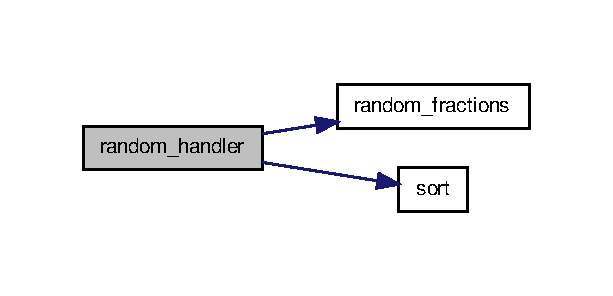
\includegraphics[width=294pt]{fraction__main_8cpp_a45ba46a5ae34b55a833eced785f695ea_cgraph}
\end{center}
\end{figure}


\hypertarget{fraction__main_8cpp_a7c827c26e5661b0c05da029a209d0cb8}{\index{fraction\-\_\-main.\-cpp@{fraction\-\_\-main.\-cpp}!show\-\_\-manual@{show\-\_\-manual}}
\index{show\-\_\-manual@{show\-\_\-manual}!fraction_main.cpp@{fraction\-\_\-main.\-cpp}}
\subsubsection[{show\-\_\-manual}]{\setlength{\rightskip}{0pt plus 5cm}void show\-\_\-manual (
\begin{DoxyParamCaption}
{}
\end{DoxyParamCaption}
)}}\label{fraction__main_8cpp_a7c827c26e5661b0c05da029a209d0cb8}
Reads the file \char`\"{}manual.\-txt\char`\"{} and prints it`s content to the console. \hypertarget{fraction__main_8cpp_a5703c295722633fe65e49e83e620c6b5}{\index{fraction\-\_\-main.\-cpp@{fraction\-\_\-main.\-cpp}!sort@{sort}}
\index{sort@{sort}!fraction_main.cpp@{fraction\-\_\-main.\-cpp}}
\subsubsection[{sort}]{\setlength{\rightskip}{0pt plus 5cm}void sort (
\begin{DoxyParamCaption}
\item[{std\-::vector$<$ {\bf Fraction} $>$ \&}]{fractions, }
\item[{int}]{length, }
\item[{bool}]{asc}
\end{DoxyParamCaption}
)}}\label{fraction__main_8cpp_a5703c295722633fe65e49e83e620c6b5}
Sorts an vector of fractions with the entry sort algorithm in according to the param asc ascendent or descendent.


\begin{DoxyParams}{Parameters}
{\em fractions} & Vector with the fraction to sort. \\
\hline
{\em length} & Length of the vector. \\
\hline
{\em asc} & Direction to sort. true =$>$ asc, false =$>$ desc. \\
\hline
\end{DoxyParams}

\hypertarget{fraction__main_8h}{\section{fraction\-\_\-main.\-h File Reference}
\label{fraction__main_8h}\index{fraction\-\_\-main.\-h@{fraction\-\_\-main.\-h}}
}
{\ttfamily \#include \char`\"{}fraction.\-h\char`\"{}}\\*
{\ttfamily \#include $<$string$>$}\\*
{\ttfamily \#include $<$vector$>$}\\*
Include dependency graph for fraction\-\_\-main.\-h\-:\nopagebreak
\begin{figure}[H]
\begin{center}
\leavevmode
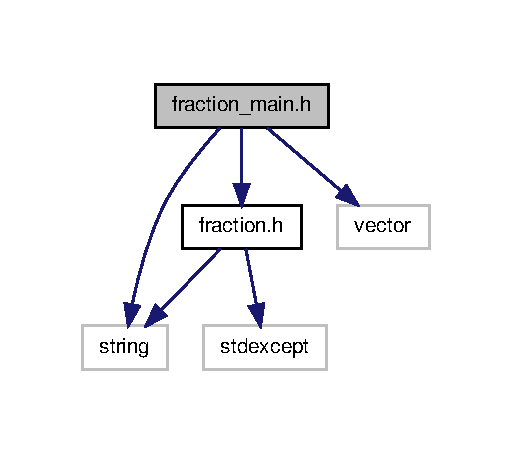
\includegraphics[width=246pt]{fraction__main_8h__incl}
\end{center}
\end{figure}
This graph shows which files directly or indirectly include this file\-:\nopagebreak
\begin{figure}[H]
\begin{center}
\leavevmode
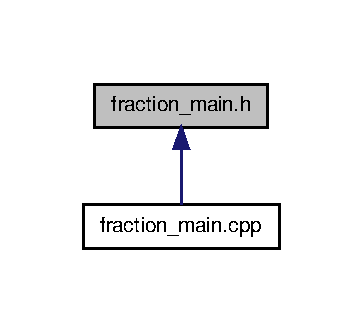
\includegraphics[width=174pt]{fraction__main_8h__dep__incl}
\end{center}
\end{figure}
\subsection*{Typedefs}
\begin{DoxyCompactItemize}
\item 
typedef \hyperlink{classFraction}{Fraction}(Fraction\-::$\ast$ \hyperlink{fraction__main_8h_a9b6408a5e81c4f9a51ed827e8c7ca6b3}{fptr} )(const \hyperlink{classFraction}{Fraction} \&) const 
\item 
typedef \hyperlink{classFraction}{Fraction}(Fraction\-::$\ast$ \hyperlink{fraction__main_8h_a418b3bd910bac84dd93361a1c0400690}{fptr2} )(const int \&) const 
\item 
typedef \hyperlink{classFraction}{Fraction}($\ast$ \hyperlink{fraction__main_8h_aa046d174f627935ab5810e02c246e7b3}{fptr3} )(const int \&, const \hyperlink{classFraction}{Fraction} \&)
\end{DoxyCompactItemize}
\subsection*{Functions}
\begin{DoxyCompactItemize}
\item 
void \hyperlink{fraction__main_8h_a88a5a1f559a0f664dbb99b66f6c86c59}{handle\-\_\-five} (char $\ast$argv\mbox{[}$\,$\mbox{]})
\item 
void \hyperlink{fraction__main_8h_afbc888f515c7c31845c525098c70a949}{handle\-\_\-six} (char $\ast$argv\mbox{[}$\,$\mbox{]})
\item 
void \hyperlink{fraction__main_8h_a6d598685a1aa70dc69dc3d66f694415d}{handle\-\_\-nine} (char $\ast$argv\mbox{[}$\,$\mbox{]})
\item 
void \hyperlink{fraction__main_8h_a24574ed2cace07e9d96f9cf8c14e9fa6}{sort} (std\-::vector$<$ \hyperlink{classFraction}{Fraction} $>$ \&array, int length, bool asc)
\item 
std\-::vector$<$ \hyperlink{classFraction}{Fraction} $>$ \hyperlink{fraction__main_8h_a7bc0d7d99bb9ae80f7ab54fcd1d3da01}{random\-\_\-fractions} (int amounth, int low\-\_\-numerator, int low\-\_\-denominator, int high\-\_\-numerator, int high\-\_\-denominator)  throw (const std\-::invalid\-\_\-argument)
\item 
void \hyperlink{fraction__main_8h_a45ba46a5ae34b55a833eced785f695ea}{random\-\_\-handler} (int n, int a, int b, int c, int d, bool asc)
\item 
bool \hyperlink{fraction__main_8h_a1920cd03342937f72cb6c49041a6953d}{isi} (char text\mbox{[}$\,$\mbox{]})
\item 
void \hyperlink{fraction__main_8h_a7c827c26e5661b0c05da029a209d0cb8}{show\-\_\-manual} ()
\end{DoxyCompactItemize}


\subsection{Typedef Documentation}
\hypertarget{fraction__main_8h_a9b6408a5e81c4f9a51ed827e8c7ca6b3}{\index{fraction\-\_\-main.\-h@{fraction\-\_\-main.\-h}!fptr@{fptr}}
\index{fptr@{fptr}!fraction_main.h@{fraction\-\_\-main.\-h}}
\subsubsection[{fptr}]{\setlength{\rightskip}{0pt plus 5cm}typedef {\bf Fraction}(Fraction\-::$\ast$ fptr)(const {\bf Fraction} \&) const }}\label{fraction__main_8h_a9b6408a5e81c4f9a51ed827e8c7ca6b3}
\hypertarget{fraction__main_8h_a418b3bd910bac84dd93361a1c0400690}{\index{fraction\-\_\-main.\-h@{fraction\-\_\-main.\-h}!fptr2@{fptr2}}
\index{fptr2@{fptr2}!fraction_main.h@{fraction\-\_\-main.\-h}}
\subsubsection[{fptr2}]{\setlength{\rightskip}{0pt plus 5cm}typedef {\bf Fraction}(Fraction\-::$\ast$ fptr2)(const int \&) const }}\label{fraction__main_8h_a418b3bd910bac84dd93361a1c0400690}
\hypertarget{fraction__main_8h_aa046d174f627935ab5810e02c246e7b3}{\index{fraction\-\_\-main.\-h@{fraction\-\_\-main.\-h}!fptr3@{fptr3}}
\index{fptr3@{fptr3}!fraction_main.h@{fraction\-\_\-main.\-h}}
\subsubsection[{fptr3}]{\setlength{\rightskip}{0pt plus 5cm}typedef {\bf Fraction}($\ast$ fptr3)(const int \&, const {\bf Fraction} \&)}}\label{fraction__main_8h_aa046d174f627935ab5810e02c246e7b3}


\subsection{Function Documentation}
\hypertarget{fraction__main_8h_a88a5a1f559a0f664dbb99b66f6c86c59}{\index{fraction\-\_\-main.\-h@{fraction\-\_\-main.\-h}!handle\-\_\-five@{handle\-\_\-five}}
\index{handle\-\_\-five@{handle\-\_\-five}!fraction_main.h@{fraction\-\_\-main.\-h}}
\subsubsection[{handle\-\_\-five}]{\setlength{\rightskip}{0pt plus 5cm}void handle\-\_\-five (
\begin{DoxyParamCaption}
\item[{char $\ast$}]{argv\mbox{[}$\,$\mbox{]}}
\end{DoxyParamCaption}
)}}\label{fraction__main_8h_a88a5a1f559a0f664dbb99b66f6c86c59}
Handles program when executed with five arguments. Validates input format.

Possible actions are\-: bruch a op c d a op c/d = e/f =$>$ bruch 1 -\/ 1 2 1 -\/ 1/2 = 1/2 bruch a b op c a/b op c = e/f =$>$ bruch 1 2 -\/ 1 1/2 -\/ 1 = -\/1/2


\begin{DoxyParams}{Parameters}
{\em $\ast$argv\mbox{[}$\,$\mbox{]}} & Arguments array form the program execution. \\
\hline
\end{DoxyParams}


Here is the call graph for this function\-:\nopagebreak
\begin{figure}[H]
\begin{center}
\leavevmode
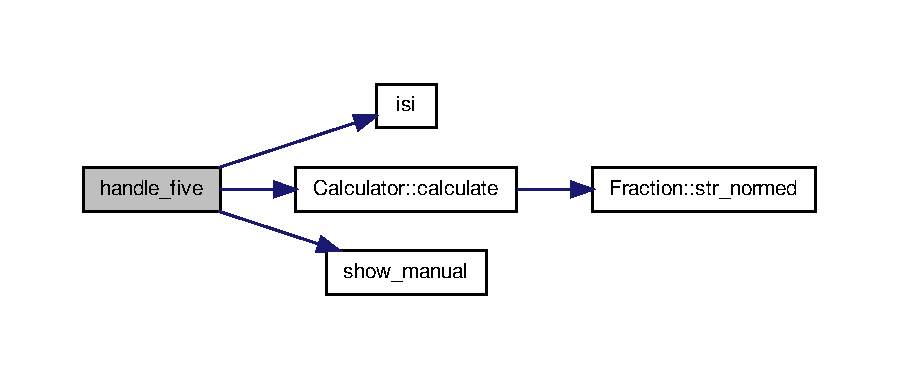
\includegraphics[width=350pt]{fraction__main_8h_a88a5a1f559a0f664dbb99b66f6c86c59_cgraph}
\end{center}
\end{figure}


\hypertarget{fraction__main_8h_a6d598685a1aa70dc69dc3d66f694415d}{\index{fraction\-\_\-main.\-h@{fraction\-\_\-main.\-h}!handle\-\_\-nine@{handle\-\_\-nine}}
\index{handle\-\_\-nine@{handle\-\_\-nine}!fraction_main.h@{fraction\-\_\-main.\-h}}
\subsubsection[{handle\-\_\-nine}]{\setlength{\rightskip}{0pt plus 5cm}void handle\-\_\-nine (
\begin{DoxyParamCaption}
\item[{char $\ast$}]{argv\mbox{[}$\,$\mbox{]}}
\end{DoxyParamCaption}
)}}\label{fraction__main_8h_a6d598685a1aa70dc69dc3d66f694415d}
Handles program when executed with nine arguments. Validates input format.

Possible actions are\-: bruch n \mbox{[} a b c d \mbox{]} + n numbers between a/b and c/d ascendent sorted. bruch n \mbox{[} a b c d \mbox{]} -\/ n numbers between a/b and c/d descendent sorted.


\begin{DoxyParams}{Parameters}
{\em $\ast$argv\mbox{[}$\,$\mbox{]}} & Arguments array form the program execution. \\
\hline
\end{DoxyParams}


Here is the call graph for this function\-:\nopagebreak
\begin{figure}[H]
\begin{center}
\leavevmode
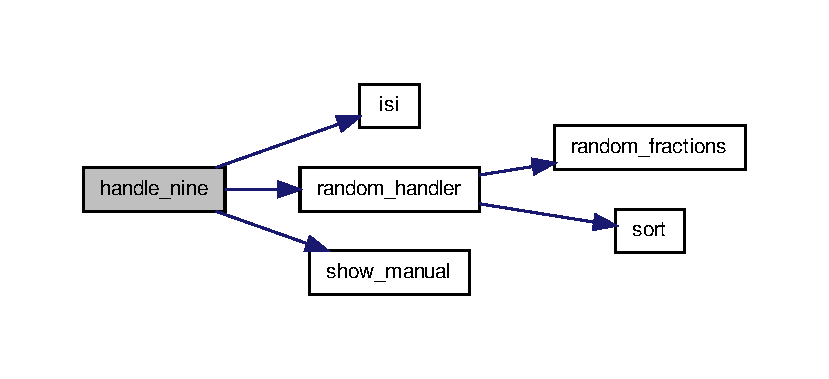
\includegraphics[width=350pt]{fraction__main_8h_a6d598685a1aa70dc69dc3d66f694415d_cgraph}
\end{center}
\end{figure}


\hypertarget{fraction__main_8h_afbc888f515c7c31845c525098c70a949}{\index{fraction\-\_\-main.\-h@{fraction\-\_\-main.\-h}!handle\-\_\-six@{handle\-\_\-six}}
\index{handle\-\_\-six@{handle\-\_\-six}!fraction_main.h@{fraction\-\_\-main.\-h}}
\subsubsection[{handle\-\_\-six}]{\setlength{\rightskip}{0pt plus 5cm}void handle\-\_\-six (
\begin{DoxyParamCaption}
\item[{char $\ast$}]{argv\mbox{[}$\,$\mbox{]}}
\end{DoxyParamCaption}
)}}\label{fraction__main_8h_afbc888f515c7c31845c525098c70a949}
Handles program when executed with six arguments. Validates input format.

Possible actions are\-: bruch a b op c d a/b op c/d = e/f =$>$ bruch 1 2 -\/ 1 3 1/2 -\/ 1/3 = 1/6 bruch a b -\/v c d a/b \mbox{[}$<$$|$$>$$|$=\mbox{]} c/d =$>$ 1 2 -\/v 1 3 1/2 $>$ 1/3


\begin{DoxyParams}{Parameters}
{\em $\ast$argv\mbox{[}$\,$\mbox{]}} & Arguments array form the program execution. \\
\hline
\end{DoxyParams}


Here is the call graph for this function\-:\nopagebreak
\begin{figure}[H]
\begin{center}
\leavevmode
\includegraphics[width=350pt]{fraction__main_8h_afbc888f515c7c31845c525098c70a949_cgraph}
\end{center}
\end{figure}


\hypertarget{fraction__main_8h_a1920cd03342937f72cb6c49041a6953d}{\index{fraction\-\_\-main.\-h@{fraction\-\_\-main.\-h}!isi@{isi}}
\index{isi@{isi}!fraction_main.h@{fraction\-\_\-main.\-h}}
\subsubsection[{isi}]{\setlength{\rightskip}{0pt plus 5cm}bool isi (
\begin{DoxyParamCaption}
\item[{char}]{text\mbox{[}$\,$\mbox{]}}
\end{DoxyParamCaption}
)}}\label{fraction__main_8h_a1920cd03342937f72cb6c49041a6953d}
Checks whether an array of chars represents an integer or not. Solfs atoi problem that returns a 0 for a char which is not a number.


\begin{DoxyParams}{Parameters}
{\em text\mbox{[}$\,$\mbox{]}} & Array of chars.\\
\hline
\end{DoxyParams}
\begin{DoxyReturn}{Returns}
true when text\mbox{[}\mbox{]} represents a number. false when text\mbox{[}\mbox{]} doesn't represent a number. 
\end{DoxyReturn}
\hypertarget{fraction__main_8h_a7bc0d7d99bb9ae80f7ab54fcd1d3da01}{\index{fraction\-\_\-main.\-h@{fraction\-\_\-main.\-h}!random\-\_\-fractions@{random\-\_\-fractions}}
\index{random\-\_\-fractions@{random\-\_\-fractions}!fraction_main.h@{fraction\-\_\-main.\-h}}
\subsubsection[{random\-\_\-fractions}]{\setlength{\rightskip}{0pt plus 5cm}std\-::vector$<${\bf Fraction}$>$ random\-\_\-fractions (
\begin{DoxyParamCaption}
\item[{int}]{n, }
\item[{int}]{low\-\_\-numerator, }
\item[{int}]{low\-\_\-denominator, }
\item[{int}]{high\-\_\-numerator, }
\item[{int}]{high\-\_\-denominator}
\end{DoxyParamCaption}
)  throw (const std\-::invalid\-\_\-argument)}}\label{fraction__main_8h_a7bc0d7d99bb9ae80f7ab54fcd1d3da01}
Generates n random Fractions with value in between the Fractions a/b and c/d and gives them back as vector.


\begin{DoxyParams}{Parameters}
{\em n} & Number of random fractions. \\
\hline
{\em low\-\_\-numerator} & Numerator of the low bound fraction. \\
\hline
{\em low\-\_\-denominator} & Denominator of the low bound fraction. \\
\hline
{\em high\-\_\-numerator} & Numerator of the high bound fraction. \\
\hline
{\em high\-\_\-denominator} & Denominator of the high bound fraction.\\
\hline
\end{DoxyParams}
\begin{DoxyReturn}{Returns}
vector with the fractions. 
\end{DoxyReturn}
\hypertarget{fraction__main_8h_a45ba46a5ae34b55a833eced785f695ea}{\index{fraction\-\_\-main.\-h@{fraction\-\_\-main.\-h}!random\-\_\-handler@{random\-\_\-handler}}
\index{random\-\_\-handler@{random\-\_\-handler}!fraction_main.h@{fraction\-\_\-main.\-h}}
\subsubsection[{random\-\_\-handler}]{\setlength{\rightskip}{0pt plus 5cm}void random\-\_\-handler (
\begin{DoxyParamCaption}
\item[{int}]{n, }
\item[{int}]{a, }
\item[{int}]{b, }
\item[{int}]{c, }
\item[{int}]{d, }
\item[{bool}]{asc}
\end{DoxyParamCaption}
)}}\label{fraction__main_8h_a45ba46a5ae34b55a833eced785f695ea}
Generates n random Fractions in between the Fractions a/b and c/d, sorts them eigther ascendent or descendent according the parameter asc and prints the sorted and unsorted result to the console.


\begin{DoxyParams}{Parameters}
{\em n} & Number of random fractions. \\
\hline
{\em a} & Numerator of the low bound fraction. \\
\hline
{\em b} & Denominator of the low bound fraction. \\
\hline
{\em c} & Numerator of the high bound fraction. \\
\hline
{\em d} & Denominator of the high bound fraction. \\
\hline
{\em asc} & Deriction to sort, true =$>$ asc, false =$>$ desc. \\
\hline
\end{DoxyParams}


Here is the call graph for this function\-:\nopagebreak
\begin{figure}[H]
\begin{center}
\leavevmode
\includegraphics[width=294pt]{fraction__main_8h_a45ba46a5ae34b55a833eced785f695ea_cgraph}
\end{center}
\end{figure}


\hypertarget{fraction__main_8h_a7c827c26e5661b0c05da029a209d0cb8}{\index{fraction\-\_\-main.\-h@{fraction\-\_\-main.\-h}!show\-\_\-manual@{show\-\_\-manual}}
\index{show\-\_\-manual@{show\-\_\-manual}!fraction_main.h@{fraction\-\_\-main.\-h}}
\subsubsection[{show\-\_\-manual}]{\setlength{\rightskip}{0pt plus 5cm}void show\-\_\-manual (
\begin{DoxyParamCaption}
{}
\end{DoxyParamCaption}
)}}\label{fraction__main_8h_a7c827c26e5661b0c05da029a209d0cb8}
Reads the file \char`\"{}manual.\-txt\char`\"{} and prints it`s content to the console. \hypertarget{fraction__main_8h_a24574ed2cace07e9d96f9cf8c14e9fa6}{\index{fraction\-\_\-main.\-h@{fraction\-\_\-main.\-h}!sort@{sort}}
\index{sort@{sort}!fraction_main.h@{fraction\-\_\-main.\-h}}
\subsubsection[{sort}]{\setlength{\rightskip}{0pt plus 5cm}void sort (
\begin{DoxyParamCaption}
\item[{std\-::vector$<$ {\bf Fraction} $>$ \&}]{fractions, }
\item[{int}]{length, }
\item[{bool}]{asc}
\end{DoxyParamCaption}
)}}\label{fraction__main_8h_a24574ed2cace07e9d96f9cf8c14e9fa6}
Sorts an vector of fractions with the entry sort algorithm in according to the param asc ascendent or descendent.


\begin{DoxyParams}{Parameters}
{\em fractions} & Vector with the fraction to sort. \\
\hline
{\em length} & Length of the vector. \\
\hline
{\em asc} & Direction to sort. true =$>$ asc, false =$>$ desc. \\
\hline
\end{DoxyParams}

\addcontentsline{toc}{part}{Index}
\printindex
\end{document}
